\documentclass[12pt]{article}

\usepackage{svg}
\svgpath{{img/}}
\usepackage{wrapfig}
\usepackage{caption}
\usepackage{subcaption}
\usepackage{float}

\usepackage[T2A]{fontenc}
\usepackage[utf8]{inputenc}
\usepackage[english,russian]{babel}

\usepackage{amsmath}
\usepackage{amsthm, mathrsfs, mathtools, amssymb}
\usepackage{enumitem}

\usepackage{physics}

\usepackage{epigraph}

\usepackage{tikz}
\usepackage{subcaption}
\usepackage{caption}
\usepackage{tensor}
\usepackage{float}
\usepackage{multirow}
\usepackage{multicol}
\usepackage{wrapfig}
\usepackage{hyperref}
\hypersetup{
	colorlinks,
	citecolor=black,
	filecolor=black,
	linkcolor=black,
	urlcolor=black
}
\usepackage{titlesec}
\DeclareMathOperator{\supp}{supp}

\usepackage{geometry}
\geometry{verbose,a4paper,tmargin=1cm,bmargin=2cm,lmargin=1.5cm,rmargin=1.5cm}

\newtheoremstyle{example}% name
{0.7cm}% Space above
{0.7cm}% Space below
{\small}% Body font
{}% Indent amount
{\small\scshape}% Theorem head font
{.}% Punctuation after theorem head
{.5em}% Space after theorem head
{}% Theorem head spec (can be left empty, meaning ‘normal’)

\theoremstyle{example}
\newtheorem{example}{Пример}

\theoremstyle{plain}
\newtheorem{theorem}{Теорема}
\newtheorem*{theorem*}{Теорема}
\newtheorem{axiom}{Аксиома}
\newtheorem*{axiom*}{Аксиома}
\newtheorem{corollary}{Следствие}
\newtheorem*{corollary*}{Следствие} 
\newtheorem{lemma}{Лемма}
\newtheorem{utv}{Утверждение}
\newtheorem*{utv*}{Утверждение}

\theoremstyle{definition}
\newtheorem{definition}{Определение}
\newtheorem*{definition*}{Определение}
\newtheorem{question}{Вопрос}

\theoremstyle{remark}
\newtheorem{remark}{Замечание}
\newtheorem*{remark*}{Замечание}
\numberwithin{remark}{section}

\frenchspacing

\usepackage[labelsep=period]{caption}
\captionsetup{font = small}

\newcommand{\Hom}{\mathrm{Hom}}
\newcommand{\Spl}{\mathrm{Spl}}
\newcommand{\spl}{\mathrm{spl}}

\DeclareMathAlphabet{\mathbfit}{OML}{cmm}{b}{it}


\newcounter{problem} 
\newenvironment{problem}[1][]
{
	\refstepcounter{problem} 
	\par \vspace{0.7em} \noindent
	\textbf{Задача \theproblem}\ifx&#1&\else\ (#1)\fi. 
}
{
	\vspace{1em}	
}

\newenvironment{solution}
{
	\vspace{0.3em}
	\par\textsc{Решение.}
}
{
	\qed
}

\newcommand{\que}[1]{%
	\subsection{#1}
}
\renewcommand{\thesubsection}{\arabic{subsection}}

\titleformat{\section}{\centering\LARGE\bf\scshape}{}{1em}{}

\begin{document}
%	\tableofcontents 
	
	\begin{center}
		\Huge \bf	
		\textsc{Механика сплошных сред}
		\rule{\textwidth}{0.4pt}
	\end{center}
	
	\tableofcontents\newpage
  % Элементы тензорного исчисления
  \que{Локальные  векторные базисы, метрические матрицы, преобразования  координат.}


\paragraph{ Координаты и локальные векторы базиса. Локальные векторные базисы, метрические матрицы, преобразования координат.}
Введем в трехмерном пространстве прямоугольную декартову систему координат $x^i, і= 1, 2, 3$ с началом в точке 0, тогда каждой точке пространства $М$ будет взаимооднозначно соответствовать радиус-вектор $х$ с началом в точке $O$ и концом в точке $М$. Выберем такой ортонормированный базис $\bar{\textbf{e}}_i$, укоторого линии действия векторов совпадают с осями $Ox^i$, а начало -- с точкой $О$ декартовой системы координат. Такой базис будем называть декартовым. Радиус-вектор $x$ всегда можно разложить по базису $\bar{\textbf{e}}_i$:

\begin{equation*}
    \textbf{x} = x^i\bar{\textbf{e}}_i
\end{equation*}
где $x^i$ - координаты точки $М$ в декартовой системе координат. Трехмерное пространство, в котором существует единая для всех точек прямоугольная декартова система координат, называют трехмерным евклидовым.
Введем криволинейные координаты $X^i$, которые связаны с $x^i$ функциями вида:
\begin{equation*}
    \textbf{x} = \textbf{x}(X^j)
\end{equation*}
Тогда радиус-вектор точки $М$ может быть представлен как функция координат 
$X^j$:
\begin{equation*}
    x^i = x^i(X^j)
\end{equation*}
Будем далее предполагать, что функции $x^i$ непрерывно дифференцируемы и взаимнооднозначны, тогда их можно обратить:
\begin{equation*}
    X^j = X^j(x_i)
\end{equation*}
Ввиду дифференцируемости функций $\textbf{x}$ можно ввести производные:

\begin{equation*}
    \textbf{R}_j = \partial\textbf{x}/\partial X^j
\end{equation*}
которые образуют векторы, назваемые локальными векторами базиса. Эти векторы в $\textbf{R}_j$ образуют \textit{локальные вектора базиса}, они направлены по касательным к координатнымлиниям $X_j=const$ вточке $М$.
Вотличие от $\bar{\textbf{e}}_i$, векторы базиса $\textbf{R}_j$  меняются при переходе от одной точки $М$ к другой $М'$.
Заметим, что хотя формально $\bar{\textbf{e}}_i$, и $\textbf{R}_j$ определялись вразных точках, их можно привести к одной точке, так как векторы $\bar{\textbf{e}}_i$, являются свободными.


\paragraph {Якобиевы матрицы}
Можно связать векторы базисов $\bar{\textbf{e}}_i$, и $\textbf{R}_j$  Из (\textbf{?????}) и (\textbf{?????}) находим выражение:
\begin{equation*}
    \textbf{R}_j = \frac{\partial\textbf{x}}{\partial X^j} = \frac{\partial x^i}{\partial X^j} \bar{\textbf{e}}_i = Q^i_j \bar{\textbf{e}}_i
\end{equation*}
где введен объект $\bar{Q}^j_i$ с двумя индексами
\begin{equation}\label{jacobi-matrix}
    \bar{Q}^j_i= \frac{\partial x^j}{\partial X^i}
\end{equation}
Такие объекты всегда можно записать в виде матрицы. Матрицу \eqref{jacobi-matrix} называют матрицей преобразования или якобиевой матрицей.

В силу взамной однозначности функций (\textbf{?????}), в любой точке $X^i$ детерминант якобиевой матрицы всегда отличен от нуля:
\begin{equation*}
	\textbf{????}
\end{equation*}

Обратную матрицу будем также иногда обозначать как 
\begin{equation*}
    \bar{P}^i_j\bar{Q}^j_k = \bar{Q}^j_i\bar{P}^j_k  = \delta^i_k
\end{equation*}
где $\delta^i_k$ смешанный символ Кронекера
\begin{equation*}
    \delta^i_k = \begin{cases}
    1, i = k\\
    0, i \ne k
    \end{cases}
\end{equation*}
Также обозначают
\begin{equation*}
    \bar{P}^i_j= (\bar{Q^{-1}})^i_j   = (\bar{Q}^i_j)^{-1} 
\end{equation*}
Введем также ковариантный символ Кронекера $\delta_{ik}$  и контравариантный символ Кронекера $\delta^{ik}$ , значения которых совладают с $\delta^i_k$ :
\begin{equation*}
	\textbf{????}
\end{equation*}

Для якобиевой матрицы $\bar{Q}^j_i$ обратная акобиева матрица имеет вид:
\begin{equation*}
    \bar{P}^j_i= \frac{\partial X^j}{\partial x^i}
\end{equation*}
Спомощью $\bar{P}^j_i$, можно выразить векторы декартова базиса $e_k$ через $\textbf{R}_i$ . Домножая (1.6) на $\bar{P}^i_k$, получаем
\begin{equation*}
    e_k = \bar{P}^i_k \textbf{R}_i
\end{equation*}
\paragraph{Метрические матрицы}
В силу ортонормированности векторов е;, их скалярное произведе- ние можно записать с помощью символов Кронекера:
\begin{equation*}
    \bar{\textbf{e}}_k \cdot \bar{\textbf{e}}_j = \delta_{kj}
\end{equation*}
Тогда скалярное произведение векторов $\textbf{R}_i, \textbf{R}_j$ с помощью уравнений (\textbf{?????}) и (\textbf{?????}) можно представить в виде:
\begin{equation*}
    \textbf{R}_i\cdot \textbf{R}_j = 
    \bar{Q}^k_i \bar{Q}^l_j \bar{\textbf{e}}_k \bar{\textbf{e}}_l =
    \bar{Q}^k_i \bar{Q}^l_j \delta_{kl} =
    g_{ij}
\end{equation*}
 Матрица $g_{ij}$, введенная по формуле (\textbf{?????}), называется
метрической или фундаментальной.

Определитель метрической матрицы обозначим следующим образом:
\begin{equation*}
    g = \det(g_{ij}) = (\det(\bar{Q}^k_i))^2
\end{equation*}
Метрическая матрица, очевидно, является симметричной по индексам $і,j$;

В силу (\textbf{?????}) всегда $g \ne 0$, поэтому для $g_{ij}$; всегда существует обратная метрическая матрица $g^{kl}$
Непосредственной подстановкой выражения $g_{ij} = \bar{Q}^k_i \bar{Q}^l_j \delta_{kl}$ в (\textbf{?????}) можно убедиться в том, что обратная метрическая матрица $g^{ij}$ выражается через обратную матрицу Якоби:
\begin{equation*}
    g^{ij} = \bar{P}^i_k \bar{P}^j_l \delta^{kl}
\end{equation*}
\paragraph{Векторы взаимного базиса}
 помощью $g^{ij}$ определяем векторы локального взаимного базиса $\textbf{R}_i =g^{ik}\textbf{R}_k$
(\textbf{?????})
\begin{equation*}
    \textbf{R}_i = \delta^k_i\textbf{R}_k =
    g^{kl}g_{li}\textbf{R}_k = g_{li}\textbf{R}^l
\end{equation*}
  \que{Диадные  базисы, алгебраическое определение  тензора, геометрическое представление тензора }

  \que{Алгебраические операции с  тензорами, геометрическое представление операций с тензорами.}

\paragraph{Изменение компонент тензоров при замене базиса}

Пусть в пространстве $\mathcal{L}$ выбран новый базис $\mathbf{e}'_i$, связанный с базисом $\mathbf{e}_i$ матрицей преобразования $\tensor{P}{^j_i}$. Очевидно, что на основе $\mathbf{e}'_i$, так же, как на основе $\mathbf{e}_i$, можно образовать базисные диады $\mathbf{e}'_i\otimes\mathbf{e}'_k$. Установим связть между $\mathbf{e}'_i\otimes\mathbf{e}'_k$ и $\mathbf{e}_i\otimes\mathbf{e}_k$.

\begin{equation*}
	\mathbf{a}_i = \mathbf{e}'_i = \tensor{P}{^l_i}\mathbf{e}_l,\quad b^{[i]}_{jk}=\tensor{\delta}{^i_j}\mathbf{e}'_k,\quad i,j,k=\overline{1,\,n}.
\end{equation*}

Тогда
\begin{equation*}
	\mathbf{e}'_i\otimes\mathbf{e}'_k = \left[\mathbf{e}'_i\left(\tensor{\delta}{^i_j}\mathbf{e}'_k\right)\right] = \tensor{P}{^l_r}\delta^r_j\tensor{P}{^i_k}\mathbf{e}_l\otimes\mathbf{e}_r
\end{equation*}

Получаем формулы для связи диадных базисов:
\begin{align*}
	\mathbf{e}'_i\otimes\mathbf{e}'_k &= \tensor{P}{^l_r}\tensor{P}{^i_k}\mathbf{e}_l\otimes\mathbf{e}_i,\\
	\mathbf{e}_l\otimes\mathbf{e}_i &= \tensor{Q}{^j_l}\tensor{Q}{^k_i}\mathbf{e}'_j\otimes\mathbf{e}'_k
\end{align*}

Отсюда следует формула для связи компонент $T'^{jk}, T^{il}$:
\begin{equation*}
	T^{il} = T'^{jk}\tensor{P}{^i_j}\tensor{P}{^l_k}.
\end{equation*}

Аналогично получается формула в сопряженном пространстве:
\begin{equation*}
	T_{il} = T'_{jk}\tensor{P}{^j_i}\tensor{P}{^k_l}.
\end{equation*}

\begin{theorem}[Тензорный закон]
	Аналогичными действиями выводится формула для общего случая:
	\begin{equation*}
		\mathbf{e}'^{i_1}\otimes\dots\otimes\mathbf{e}'^{i_p}\otimes\mathbf{e}'_{i_p+1}\otimes\dots\otimes\mathbf{e}'_{i_k} = 
		\tensor{Q}{^{i_1}_{j_1}}\dots\tensor{Q}{^{i_p}_{j_p}}\tensor{P}{^{j_{p+1}}_{i_{p+1}}}\dots\tensor{P}{^{j_k}_{i_k}}\mathbf{e}^{j_1}\otimes\dots\otimes\mathbf{e}^{j_p}\otimes\mathbf{e}^{j_{p+1}}\otimes\dots\otimes\mathbf{e}^{j_k}.
	\end{equation*}
	\begin{equation*}
\tensor{T}{_{i_1\dots i_p}^{i_{p+1}\dots i_k}} = \tensor{Q}{^{j_1}_{i_1}}\dots\tensor{Q}{^{j_p}_{i_p}}\tensor{P}{^{i_{p+1}}_{j_{p+1}}}\dots\tensor{P}{^{i_k}_{j_k}}\tensor{T}{_{j_1\dots j_p}^{j_{p+1}\dots j_k}}.
	\end{equation*}
\end{theorem}

\paragraph{Сложение и умножение тензоров на число}
\textit{С этого момента я начну сокращать ибо димус пишет тысячу страниц на один микропук}

\begin{align*}
	\tensor[^k]{\mathbf{T}}{} + \tensor[^k]{\mathbf{B}}{} &= \left(
	\tensor{T}{^{{i_1}\dots{i_k}}} + \tensor{B}{^{{i_1}\dots{i_k}}}
	\right) \mathbf{e}_{i_1}\otimes\dots\otimes \mathbf{e}_{i_k},\\
	s\tensor[^k]{\mathbf{T}}{} &= \left(\phantom{ttttt}s\tensor{T}{^{{i_1}\dots{i_k}}}\:\phantom{tttt}\right)\mathbf{e}_{i_1}\otimes\dots\otimes \mathbf{e}_{i_k}
\end{align*}

\paragraph{Тензорное произведение тензоров}
Тензорным произведением двух тензоров $\tensor[^m]{\mathbf{T}}{}$ и $\tensor[^k]{\mathbf{B}}{}$:
\begin{align*}
	\tensor[^m]{\mathbf{T}}{} &= \tensor{T}{_{i_1\dots i_p}^{i_{p+1}\dots i_m}}\mathbf{e}^{i_1}\otimes\dots\otimes\mathbf{e}^{i_p}\otimes\mathbf{e}_{i_{p+1}}\otimes\dots\otimes\mathbf{e}_{i_m},\\
	\tensor[^k]{\mathbf{B}}{} &= \tensor{B}{_{i_1\dots i_{p'}}^{i_{p'+1}\dots i_k}}\mathbf{e}^{i_1}\otimes\dots\otimes\mathbf{e}^{i_{p'}}\otimes\mathbf{e}_{i_{p'+1}}\otimes\dots\otimes\mathbf{e}_{i_k},
\end{align*}
называется тензор $(m+k)$-го ранга $\tensor[^{m+k}]{\mathbf{C}}{}$:
\begin{multline*}
	\tensor[^{m+k}]{\mathbf{C}}{} = \tensor[^m]{\mathbf{T}}{}\otimes\tensor[^k]{\mathbf{B}}{}=
	\tensor{T}{_{i_1\dots i_p}^{i_{p+1}\dots i_m}}\tensor{B}{_{i_{m+1}\dots i_{m+p'}}^{i_{m+p'+1}\dots i_{m+k}}}\mathbf{e}^{i_1}\otimes\dots\otimes\mathbf{e}^{i_p}\otimes\mathbf{e}_{i_{p+1}}\otimes\dots\otimes\mathbf{e}_{i_m}\\
	\mathbf{e}^{i_{m+1}}\otimes\dots\otimes\mathbf{e}^{i_{m+p'}}\otimes\mathbf{e}_{i_{m+p'+1}}\otimes\dots\otimes\mathbf{e}_{i_{m+k}}.
\end{multline*}
\paragraph{Транспонирование тензоров}
Транспонирование:
\begin{equation*}
	\mathbf{T}^T=T^{ij}\mathbf{e}_j\otimes\mathbf{e}_i=T^{ji}\mathbf{e}_j\otimes\mathbf{e}_i
\end{equation*}
Иллюстрация см. Рисунок \ref{fig:que3}.
\begin{figure}[H]
	\centering
	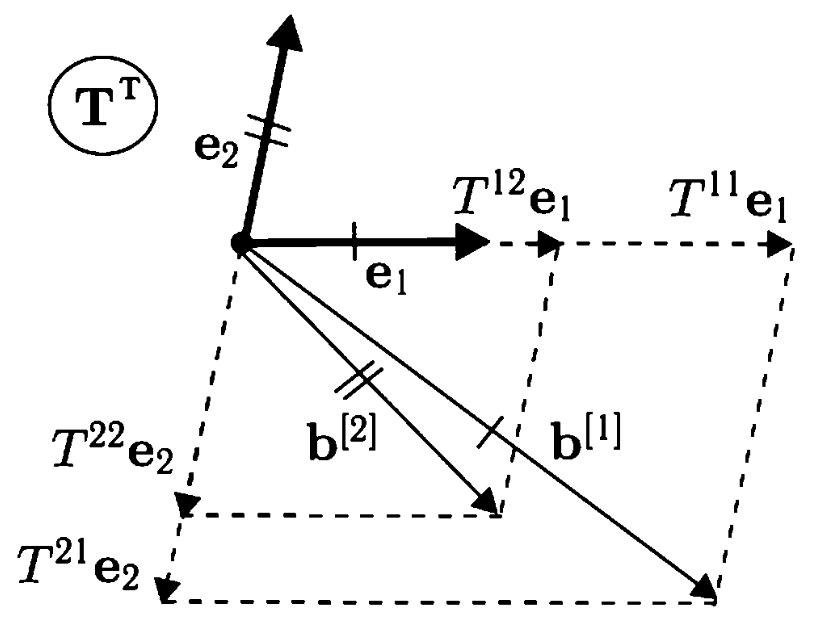
\includegraphics[width=0.5\linewidth]{img/que3}
	\caption{Геометрическое изображение тензора $\mathbf{T}^T$, транспонированного к $\mathbf{T}$ в $E_{22}$}
	\label{fig:que3}
\end{figure}
\begin{remark}
	Для тензора $n$ порядка можно ввести $n!$ различных транспонированных тензора. (Количество возможных расстановок индексов.)
\end{remark}

\paragraph{Жонглирование индексами}
\textit{очевидно. жижки, камикадзе там.}
\paragraph{Скалярное умножение тензоров в евклидовых пространствах}
Умножение тензора на тензор:
\begin{equation*}
	\mathbf{T}\cdot\cdot\mathbf{B}=T^{ij}g_{jk}B^{kl}g_{il}
\end{equation*}
\begin{equation*}
	\mathbf{T}\cdot\mathbf{B}=\left(T^{ij}\mathbf{e}_i\otimes\mathbf{e}_j\right)\left(B^{lm}\mathbf{e}_l\otimes\mathbf{e}_m\right)=T^{ij}B^{lm}g_{jl}\mathbf{e}_i\otimes\mathbf{e}_m
\end{equation*}
Умножение тензора на вектор (см. Рисунок \ref{fig:que32}):
\begin{align*}
	\mathbf{T}\cdot\mathbf{c}&=T^{ik}c_k\mathbf{e}_i,\, \text{см. Рисунок \ref{fig:que32_ten_vec}},\\
	\mathbf{C}\cdot\mathbf{T}&=c_kT^{kj}\mathbf{e}_j,\, \text{см. Рисунок \ref{fig:que32_vec_ten}}.\\
\end{align*}
\begin{figure}[H]
	\hfill
	\begin{subfigure}{0.48\textwidth}
		\centering
		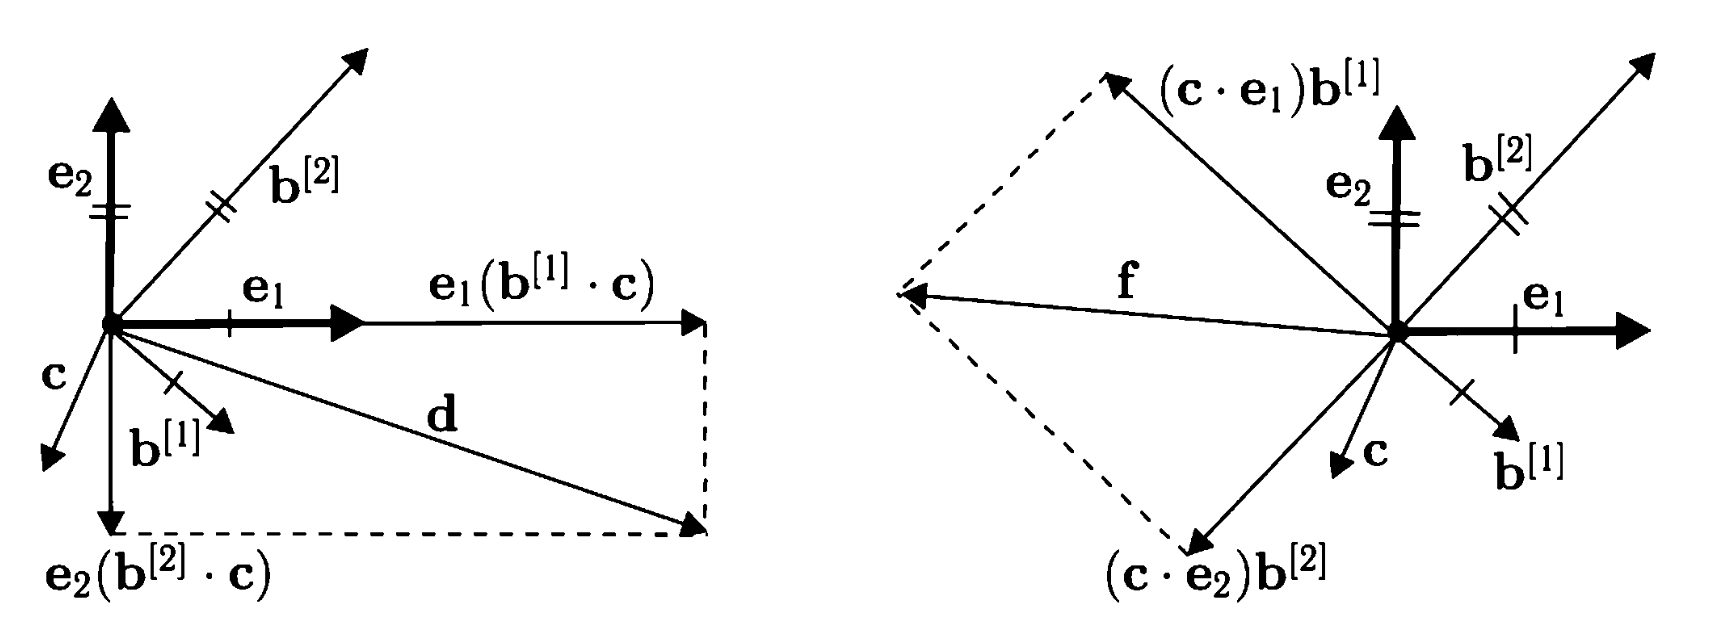
\includegraphics[width=0.7\linewidth,trim={0 0 12cm 0},clip]{img/que3_2}
		\subcaption{Геометрическое изображение скалярного произведения тензора на вектор справа: $\mathbf{T}\cdot\mathbf{c}$}
		\label{fig:que32_ten_vec}
	\end{subfigure}
	\hfill
	\begin{subfigure}{0.48\textwidth}
		\centering
		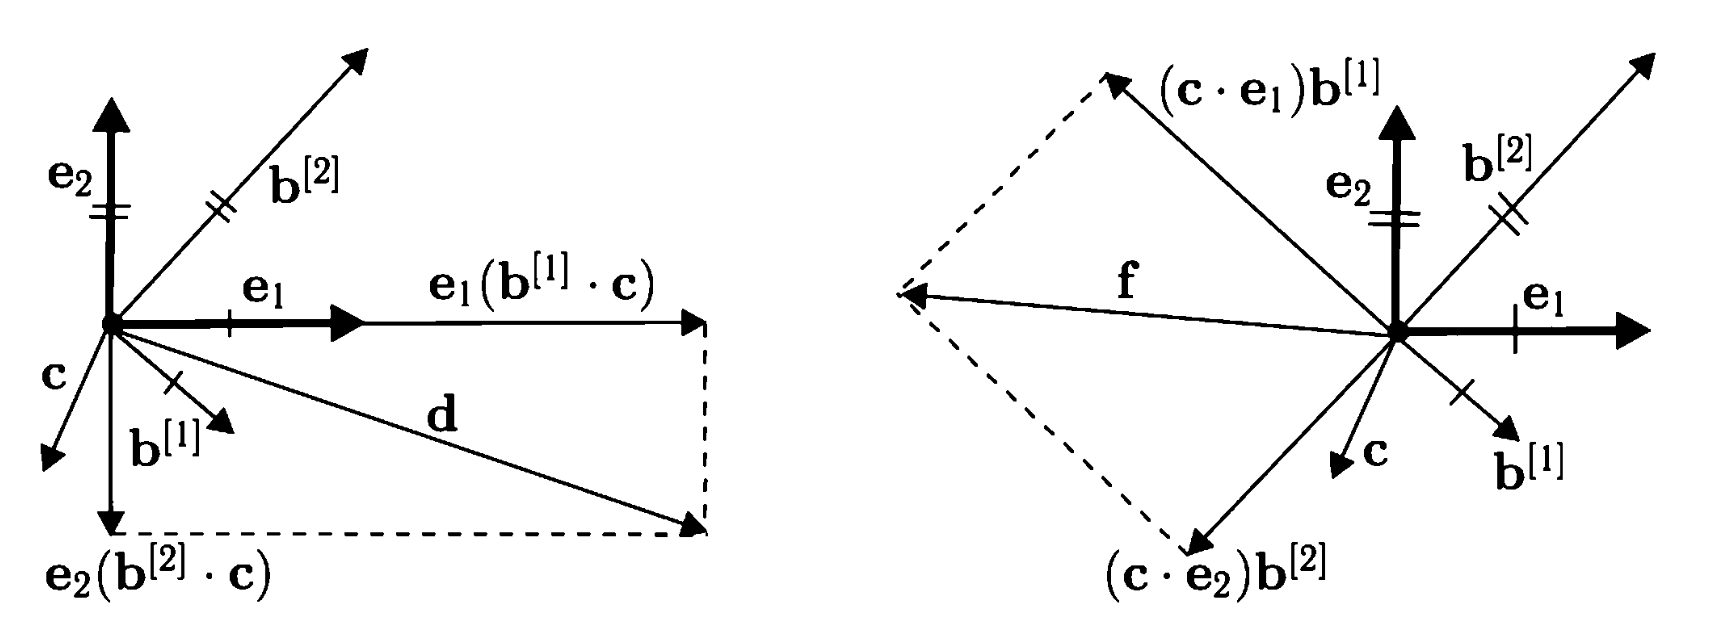
\includegraphics[width=0.7\linewidth,trim={11cm 0 0cm 0},clip]{img/que3_2}
		\subcaption{Геометрическое изображение скалярного произведения вектора на тензор слева: $\mathbf{C}\cdot\mathbf{T}$}
		\label{fig:que32_vec_ten}
	\end{subfigure}
	\hfill
	\caption{Скалярное умножение тензора на вектор}
	\label{fig:que32}
\end{figure}

\begin{utv}
	Двойное скалярное умножение тензора на базисные диады $\mathbf{e}_i\otimes\mathbf{e}_j$
\begin{equation*}
	\mathbf{T}\cdot\cdot\left(\mathbf{e}_i\otimes\mathbf{e}_j\right)=\mathbf{e}_i\cdot\mathbf{T}\cdot\mathbf{e}_j = T_{ij}
\end{equation*}
даёт компоненты этого тензора в диадном базисе $\mathbf{e}^i\otimes\mathbf{e}^j$.
\begin{proof}
	\begin{equation*}
		\mathbf{T}\cdot\cdot\left(\mathbf{e}_m\otimes\mathbf{e}_k\right)= T^{ij}\left(\mathbf{e}_i\otimes\mathbf{e}_j\right)\cdot\cdot\left(\mathbf{e}_m\otimes\mathbf{e}_k\right)=T^{ij}g_{jm}g_{ik}=T_{km}
	\end{equation*}
	Аналогичный результат получается и при умножении слева на $\mathbf{e}_i$ и справа на $\mathbf{e}_j$:
	\begin{equation*}
		\mathbf{e}_i\cdot\mathbf{T}\cdot\mathbf{e}_j = \mathbf{e}_i\cdot\left(T^{mk}\mathbf{e}_m\otimes\mathbf{e}_k\right)\cdot\mathbf{e}_j=
		T^{mk}\left(\mathbf{e}_i\cdot\mathbf{e}_m\right)\otimes\left(\mathbf{e}_k\cdot\mathbf{e}_j\right)=
		T^{mk}g_{im}g_{kj}=T_{ij}.
	\end{equation*}
\end{proof}
\end{utv}
\begin{utv}[Свойства скалярного произведения]
	Для произвольных тензоров второго ранга $\mathbf{T},\mathbf{B},\mathbf{A}\in\mathcal{E}_n^{(2)}$ и вектора $\mathbf{a}\in\mathcal{E}_2$ имеют место следующие соотношения:
	\begin{itemize}
		\item $\mathbf{a}\cdot\mathbf{A}=\mathbf{A}^T\cdot\mathbf{a}$;
		\item $\left(\mathbf{A}\cdot\mathbf{B}\right)^T=\mathbf{B}^T\cdot\mathbf{A}^T$;
		\item $\left(\mathbf{A}\cdot\mathbf{T}\right)\cdot\cdot\mathbf{B}=\mathbf{A}\cdot\cdot\left(\mathbf{T}\cdot\mathbf{B}\right)=\mathbf{B}\cdot\mathbf{A}\cdot\cdot\mathbf{T}=\mathbf{T}\cdot\mathbf{B}\cdot\mathbf{A}$;
		\item $\underbrace{\mathbf{A}\cdot\ldots\cdot\mathbf{A}}_{k}=\mathbf{A}^k$
	\end{itemize}
\end{utv}

\begin{definition}[Единичный тензор 2 ранга]
	См. Рисунок \ref{fig:que33}.
	\begin{equation*}
		\mathbf{E} = \mathbf{e}_i\otimes\mathbf{e}^i = g^{ij}\mathbf{e}_i\otimes\mathbf{e}_j
	\end{equation*}
	В виде классов эквивалентности:
	\begin{equation*}
		\mathbf{E}=\left[\mathbf{e}_k\mathbf{e}^k\right]=\left[\mathbf{e}_1\mathbf{e}^1\dots\mathbf{e}_n\mathbf{e}^n\right]
	\end{equation*}
\end{definition}
\begin{figure}[H]
	\centering
	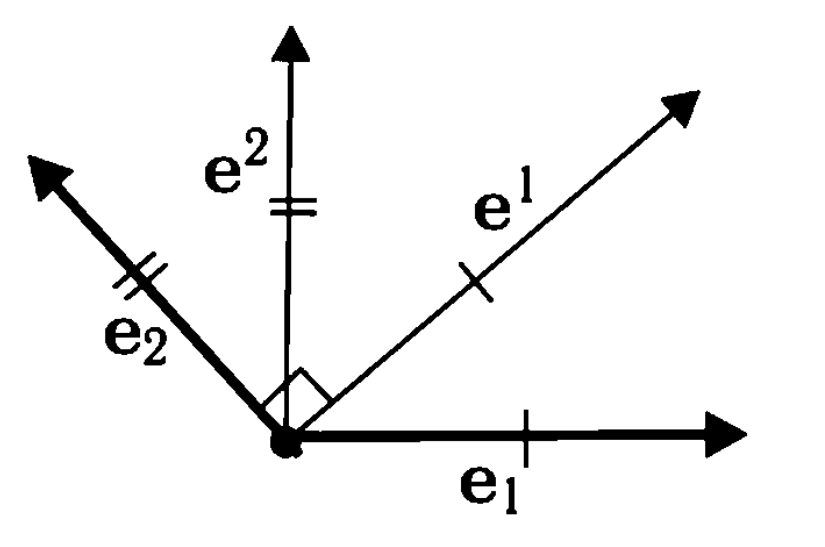
\includegraphics[width=0.4\linewidth]{img/que3_3}
	\caption{Геометрическое изображение единичного тензора в пространстве $\mathcal{E}_n^{(2)}\left(E_2\right)$}
	\label{fig:que33}
\end{figure}


  \que{Симметричные, кососимметричные и ортогональные тензоры. Собственные значения и собственные векторы тензоров 2-го ранга.}

\begin{definition}[Симметричный тензор]
	\begin{equation*}
		A=A^T,\quad A^{ij}=A^{ji}.
	\end{equation*}
\end{definition}

\begin{definition}[Кососимметричный тензор]
	\begin{equation*}
		\mathbf{A} = -\mathbf{A}^T.
	\end{equation*}
\end{definition}

\begin{definition}[Собственный вектор, собственное значение]
	Будем говорить, что $\mathbf{p}_{A\alpha}$ --- \emph{правый собственный
  вектор} для тензора второго ранга $A$, если
	он удовлетворяет уравнению $A \cdot \mathbf{p}_{A\alpha} = \lambda_{A\alpha}
  \cdot \mathbf{p}_{A\alpha}$; числа $\lambda_{A\sigma}$ будем называть
  \emph{правыми собственными значениями.}
	
  Аналогично, \emph{левым собственным вектором} называется такой вектор $\mathbf{p}^*_{A\alpha}$, что
	$\mathbf{p}^*_{A\alpha} \cdot A = \lambda^*_{A\alpha} \cdot \mathbf{p}^*_{A\alpha}$.
\end{definition}

\begin{corollary}
	Если $A$ --- симметричный, то
  \begin{itemize}[label=--]
		\item все собственные значения вещественные;
    \item все собственные векторы вещественнозначные, т.\,е. все компоненты в
      декартовом базисе
		вещественные;
		\item $\mathbf{p}_{A\alpha} = \mathbf{p}^*_{A\alpha}$;
		\item $\mathbf{p}_{A\alpha} \cdot \mathbf{p}_{A\beta} = \delta_{\alpha\beta}.$
	\end{itemize}
	
	Если он к тому же положительно определенный, то все собственные значения еще и положительны.
\end{corollary}
\begin{corollary}
	Представим симметричный тензор в собственном базисе. Если $A$ --- симметричный,
	$\mathbf{p}_{A\alpha}$ --- собственные векторы, $\lambda_{A\alpha}$ --- собственные значения,
	тогда
	\[
	A = \sum_{\alpha=1}^3 \lambda_{A\alpha} \mathbf{p}_{A\alpha} \otimes \mathbf{p}_{A\alpha}
	= A^{ij} \mathbf{r}_i \otimes \mathbf{r}_j.
	\]
	\begin{proof}
		Для доказательства подставим в определение собственных векторов для симметричного тензора:
		\[
		A \cdot \mathbf{p}_{A\alpha}
		= \sum_{\beta=1}^3 \lambda_{A\beta} (\mathbf{p}_{A\alpha}\otimes \mathbf{p}_{A\beta}) \cdot \mathbf{p}_{A\alpha}
		= \sum_{\beta=1}^3 \lambda_{A\beta} \mathbf{p}_{A\alpha} \otimes \delta_{\alpha\beta}
		% = \sum_{\beta=1}^3 \lambda_{A\beta} %TODO
		= \lambda_{A\alpha} \mathbf{p}_{A\alpha}.
		\]
	\end{proof}
\end{corollary}

\begin{definition}[Ортогональный тензор]
	\begin{equation*}
		O\in\mathcal{E}_3^{(2)}\colon O^T=O^{-1}.
	\end{equation*}
\end{definition}
Введем компоненты в диадном базисе:
\begin{equation*}
	O = \tensor{O}{^i_j}\mathbf{e}_i\otimes\mathbf{e}^j,
\end{equation*}
тогда
\begin{equation*}
	\tensor{O}{^i_j}\tensor{O}{_k^j}=\tensor{O}{^i^k}\tensor{O}{_k_j}=\delta^i_k \Leftrightarrow
	\tensor{O}{^i_j}\tensor{O}{^m_k}g_{im}=g_{jk}.
\end{equation*}
В ортонормированном базисе:
\begin{equation*}
	\tensor{O}{^i_j}\tensor{O}{^m_k}\delta_{im}=\delta_{jk}.
\end{equation*}
Определитель:
\begin{equation*}
	\left(\det O\right)^2 = \det(O^T)\det(O) = \det(O^TO)=\det E = 1 \Rightarrow \det O = \pm1
\end{equation*}
Строки и столбцы умноженные сами на себя дают единицу, а перемноженные попарно дают нуль:
\begin{equation*}
	\sum_{\alpha=1}^{3}\tensor{O}{^\alpha_\beta}^2=1,\quad\sum_{\alpha=1}^{3}\tensor{O}{^\alpha_\beta}\tensor{O}{^\alpha_\gamma}=1,\quad \alpha,\beta,\gamma=1,2,3.
\end{equation*}

Ортогональный тензор всегда имеет одно действительное собственное значение, равное 1, и два, вообще говоря, комплексных.


  \que{Векторное произведение, его свойства, символы Леви-Чивиты.}

\begin{definition}[Символ Леви-Чивиты]
	\begin{equation*}
		\epsilon_{ijk},\epsilon^{ijk} = \begin{cases}
			0, &\text{если среди $i,j,k$ есть повторения};\\
			1, &\text{если $(ijk)$ - четная подстановка};\\
			-1,&\text{если $(ijk)$ - четная подстановка}.\\
		\end{cases}
	\end{equation*}
\end{definition}

\begin{definition}[Определитель]
	Для матрицы 3х3 верна формула:
	\begin{equation*}
		\det(\tensor{A}{^i_j}) = \frac{1}{6}\epsilon_{ijk}\epsilon^{mnl}\tensor{A}{^i_m}\tensor{A}{^j_n}\tensor{A}{^k_l}.
	\end{equation*}
	(легко можно проверить подставив в лоб)
	
	Расписав покомпонентно один из символов Леви-Чевиты и упростив легко выделить другое выражение
	\begin{equation*}
		\det(\tensor{A}{^i_j}) = \epsilon_{ijk}\tensor{A}{^i_\alpha}\tensor{A}{^j_\beta}\tensor{A}{^k_\gamma},\quad \alpha\neq\beta\neq\gamma,\quad\alpha,\beta,\gamma=1,2,3.
	\end{equation*}
\end{definition}

Для метрической матрицы $g_{ij}, g^{ij}$ формулы выше также применимы, тогда получим, что:
\begin{align*}
	g &= \frac{1}{6}\epsilon^{ijk}\epsilon^{mnl}g_{mi}g_{nj}g_{kl},\\
	\sqrt{g}\epsilon_{ijk}&=\frac{1}{\sqrt{g}}\epsilon^{mnl}g_{mi}g_{nj}g_{lk}.
\end{align*}

\begin{definition}[Векторное произведение]
	Векторным произведением векторов $\mathbf{a}, \mathbf{b}$ из $\mathcal{E}_3$ называют следующий вектор $\mathbf{c}$ из $\mathcal{E}_3$:
	\begin{equation*}
		\mathbf{c} = \mathbf{a} \times \mathbf{b} = \sqrt{g} \epsilon_{ijk} a^ib^j\mathbf{e}^k = \frac{1}{\sqrt{g}}\epsilon^{ijk} a_ib_j\mathbf{e}_k
	\end{equation*}
\end{definition}

\begin{theorem}
	Для векторного произведения имеет место формула 
	\begin{equation*}
		\mathbf{a} \times \mathbf{b} = S\mathbf{n},
	\end{equation*}
	\begin{equation*}
		S = |\mathbf{a}||\mathbf{b}|\sin{\varphi},
	\end{equation*}
	где $\varphi$ угол между $\mathbf{a}$ и $\mathbf{b}$ ($0\leqslant\varphi\leqslant\pi$), а $\mathbf{n}$ единичный вектор, ортогональный к $\mathbf{a}$ и $\mathbf{b}$. Иллюстрация, см. Рисунок \ref{fig:que5}.
	
	\begin{proof}
		Если один из векторов $\mathbf{a}$ и $\mathbf{b}$ нулевой, то формула, очевидно, выполняется. Если векторы $\mathbf{a}$ и $\mathbf{b}$ коллинеарны, то же самое. Рассмотрим случай, когда $\mathbf{a}$ и $\mathbf{b}$ ненулевые и неколлинеарные.
		
		$\mathbf{a}$ и $\mathbf{b}$ ненулевые и неколлинеарные. Построим базис $\mathbf{e}'_i$ в $E_2$:
		\begin{equation*}
			\mathbf{e}'_1 = \mathbf{a},\quad\mathbf{e}'_2=\mathbf{b},\quad\mathbf{e}'_3=\mathbf{n}
		\end{equation*}
		Компоненты векторов $\mathbf{a}$ и $\mathbf{b}$ в этом базисе:
		\begin{equation*}
			a'i=\begin{pmatrix}
				1\\0\\0
			\end{pmatrix},\quad
			b'i=\begin{pmatrix}
				0\\1\\0
			\end{pmatrix},
		\end{equation*}
		а метрическая матрица:
		\begin{equation*}
			g'_{ij}=\mathbf{e}'_i\cdot\mathbf{e}'_j=\begin{pmatrix}
				|\mathbf{a}|^2            & \mathbf{a}\cdot\mathbf{b} & 0 \\
				\mathbf{a}\cdot\mathbf{b} & |\mathbf{b}|^2            & 0 \\
				0                         & 0                         & 1
			\end{pmatrix}
		\end{equation*}
		Тогда
		\begin{equation*}
			S=\sqrt{g'_{11}g'_{22}}\sin{\varphi}=\sqrt{g'_{11}g'_{22}}\sqrt{1-\cos^2{\varphi}},
		\end{equation*}
		где
		\begin{equation*}
			\cos\varphi = \frac{\mathbf{a}\cdot\mathbf{b}}{|\mathbf{a}||\mathbf{b}|}=\frac{g'_{12}}{\sqrt{g'_{11}g'_{22}}}, \quad\sqrt{1-\cos^2{\varphi}} = \sqrt{\frac{g'}{g'_{11}g'_{22}}}.
		\end{equation*}
		Таким образом
		\begin{equation*}
			S = \sqrt{g'_{11}g'_{22}}\sqrt{\frac{g'}{g'_{11}g'_{22}}} = \sqrt{g'},
		\end{equation*}
		При этом имеем
		\begin{equation}\label{vec prod}
			\mathbf{a} \times \mathbf{b} = \sqrt{g'} \epsilon_{123} a'^1b'^2\mathbf{e}'^3=\sqrt{g'}e'^3
		\end{equation}
		Подставляя в \eqref{vec prod} всё имеющееся, действительно получаем
		\begin{equation*}
			\mathbf{a} \times \mathbf{b} = S\mathbf{n}.
		\end{equation*}
	\end{proof}
\end{theorem}
\begin{figure}[ht!]
	\centering
	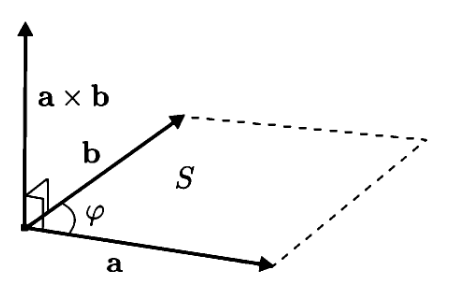
\includegraphics[width=0.5\linewidth]{img/que5}
	\caption{Геометрическое изображение векторного произведения в пространстве $E_3$}
	\label{fig:que5}
\end{figure}
\begin{theorem}[О связи векторов взимного и основного базисов в $\mathcal{E}_3$]
	Векторы взимного и основного базисов в $\mathcal{E}_3$ связаны с помощью операции векторного произведения:
	\begin{equation*}
		\mathbf{e}^\gamma = \frac{1}{\sqrt{g}}\mathbf{e}_\alpha\times\mathbf{e}_\beta,\quad\mathbf{e}_\gamma=\sqrt{g}\mathbf{e}^\alpha\times\mathbf{e}^\beta,\quad \alpha\neq\beta\neq\gamma,\quad\alpha,\beta,\gamma=1,2,3.
	\end{equation*}
	\begin{proof}
		\begin{equation*}
			\mathbf{e}_n\times\mathbf{e}_m=\sqrt{g}\epsilon_{ijk}\delta^i_n\delta^j_m\mathbf{e}^k=\sqrt{g}\epsilon_{nmk}\mathbf{e}^k
		\end{equation*}
	\end{proof}
\end{theorem}
  \que{Ковариантное дифференцирование тензоров.}

  \que{Физические  компоненты тензоров.}

Если криволинейные координаты $X^i$ являются ортогональными, то векторы $\mathring{\mathbf{r}}_i$ -- ортогональны: $ \mathring{\mathbf{r}}_i\cdot\mathring{\mathbf{r}}_j=\delta_{ij}$, а матрицы $\mathring{g}_ij$ и $\mathring{g}^ij$ -- диагональные. Тогда можно ввести параметры Ламе (см. подробнее раздел \ref{Локальные базисы и метрические матрицы в конфигурациях}.\nameref{Локальные базисы и метрические матрицы в конфигурациях}): $\mathring{H}_\alpha=\sqrt{\mathring{g_{\alpha\alpha}}},\,\alpha=1,2,3$, и \textit{физический ортонормированный базис}:
\begin{equation*}
	\widehat{\mathring{\mathbf{r}}}_\alpha=\frac{\mathring{\mathbf{r}}_\alpha}{\mathring{H}_\alpha}=\mathring{\mathbf{r}}^\alpha\mathring{H}_\alpha.
\end{equation*}
Компоненты вектора $\mathbf{a}$ в этом базисе называют физическими:
\begin{equation*}
	\mathbf{a} = \widehat{\mathring{a}}^{\,i}~\widehat{\mathring{r}}_i.
\end{equation*}

Актуальный базис $\mathbf{r}_i$ в общем случае не является ортогональным, даже если $\mathring{\mathbf{r}}_i$ -- ортогональный, поэтому нельзя ввести соответствующий ему физический базис в $\mathcal{K}$. Заметим однако, что в $\mathcal{K}$ всё-таки вводят физический базис, но по другому ... (\textit{взято из димитриенки}).

  % Кинематика сплошных сред
  \que{Лагранжево и эйлерово описания движения сплошных сред. Актуальная  и отсчетные конфигурации. Локальные базисы и метрические матрицы   в конфигурациях.}
\paragraph{Лагранжево и эйлерово описание.} Пусть дана сплошная среда $ \mathcal
P$ и некоторая её материальная точка $ \mathcal
M$ с радиусом-вектором $ \mathbf{x} $. 

Движение этой материальной точки может
рассматриваться в обычном декартовом базисе $ O\mathbf{\bar{e}}_i $, то есть как
вектор-функция $ \mathbf{x}(t) =
x^i(t)\mathbf{\bar{e}}_i  $. Такой подход к описанию движения называют
\emph{Эйлеровым}.

Другой подход состоит в том, чтобы связать с телом $ \mathcal{P} $ систему
криволинейных координат $ X^i $, которая будет <<двигаться>> вместе с телом
так, что координаты $ X^i $ точки $ \mathcal M $ в любой момент времени будут
одни и те же. Эти криволинейные координаты принадлежат телу только в случае,
если принадлежат некоторой области изменения, $ X^k \in V_X $. Этот подход
называется \emph{Лагранжевым}.

От криволинейных координат требуется регулярность, поэтому существуют следующие
соотношения: 
\[
  \mathbf{x} = \mathbf{x}(X^k, t), \qquad X^k = X^k(x^i, t).
\]
Здесь под $ X^k $ подразумевается полный набор криволинейных координат (в
трёхмерном пространстве их количество варьируется от одной до трёх).
Естественно, эти функции определены, только если $ X^k \in V_X $, $ \mathbf x \in
\mathcal P(t) $.

Соответственно, скалярные, векторные и тензорные поля (в том числе переменные)
тоже можно раскрывать как функции
криволинейных координат и времени либо же декартовых координат и времени. При
этом для твёрдых тел чаще используют лагранжево описание (следят, как меняется
фиксированная точка тела), а для жидкостей и газов --- Эйлерово (следят, как
материальные точки тела <<проходят>> через фиксированную точку пространства).

\paragraph{Актуальная и отсчётная конфигурации.} Для сплошной среды $ \mathcal P
$ определены отображения в точечно-евклидово пространство (типа строим мат. модель) $
V = V(\mathcal P, t)$, причём $ V $ является замкнутым множеством без
изолированных точек (т. н. \emph{совершенное} тело). 

Собственно, \emph{отсчётной} конфигурацией называется множество $ \mathring V =
V(\mathcal P,
0)$, а \emph{актуальной} конфигурацией --- множество $ V = V(\mathcal P, t_0) $ для
некоторого интересующего нас момента $ t_0 > 0 $.

\paragraph{Локальные базисы и метрические матрицы в конфигурациях.}\label{Локальные базисы и метрические матрицы в конфигурациях} С
криволинейными координатами $ X^i $ (точнее, с обратным отображением $ \mathbf
x(X^i) $) связана \emph{матрица Якоби} $
\tensor{Q}{^i_j} = \left( \frac{\partial x^i}{\partial X^j}\right)  $. Причём
предполагается, что Якобиан ($ \det Q $) отличен от нуля (условия регулярности),
то есть имеет обратную матрицу, которую назовём $ \tensor{P}{^i}{_j} $.
Заметим, что, вообще говоря\footnote{Если криволинейные координаты не являются
прямолинейными, то есть преобразование не линейное.}, эта матрица зависит от точки тела $ \mathcal
P$ и от времени (поскольку сами отображения $ \mathbf{x}(X^i, t) $ зависят в том
числе от времени).

Для фиксированного момента времени и точки $ \mathcal M \in \mathcal P $ назовём
столбцы этой матрицы \emph{локальным базисом} в точке $ \mathcal M $, обозн. $
\mathring{\mathbf{r}}_k $ для нулевого момента времени и $ \mathbf{r}_k $ иначе. 

Каждому локальному базису соответствует \emph{метрический тензор} $ g_{ij} =
\mathbf{r}_i \cdot \mathbf{r}_j $ (аналогично для $ \mathring g_{ij} $, далее не
подчёркивается) и
\emph{обратный метрический тензор} $ g^{ij} = g^{-1}_{ij} $. После последнего
определения нам стало доступно <<жонглирование>> индексами, в том числе
локального базиса. Именно, определим \emph{взаимный локальный базис $
\mathbf{r}^i $} по формуле $ \mathbf{r}^i = g^{ij}\mathbf{r}_j $.

Частный случай, когда векторы $ \mathbf{r}_i $ ортогональны, то есть матрица $
g_{ij} $ диагональна, дополняется определением \emph{коэффициентов Ламэ} $
H_\alpha $ как $ H_\alpha = \sqrt{g_{\alpha\alpha}} $, то есть длины
соответствующего базисного вектора.

  \que{Градиент деформаций. Тензоры деформации Альманзи и Коши-Грина. }


  \que{Физический  смысл компонент тензора  деформаций.  Преобразование ориентированной площадки при деформации сплошной среды. Геометрическая картина преобразования малой окрестности .}

  \que{Полярное разложение, тензоры искажений и поворота. Собственные значения и собственные вектора тензоров искажений.}
Очевидно, тензор $ \mathbf{F} $ невырожден.

\begin{theorem*}
Всякий невырожденный тензор второго ранга
$\mathbf{F}$ можно представить в виде скалярного произведения двух тензоров
второго ранга: \[
\mathbf{F}=\mathbf{O} \cdot \mathbf{U} \quad \text { или } \quad
\mathbf{F}=\mathbf{V} \cdot \mathbf{O}, 
\]
где $ \mathbf{U} $ и $ \mathbf{V} $ --- симметричные, положительно определенные
тензоры, а $ \mathbf{O} $ --- ортогональный тензор, причем каждое из
представлений единственное.
\end{theorem*}
\begin{proof}
Построим тензоры $\mathbf{U}, \mathbf{V}$ и $ \mathbf{O} $. Для этого рассмотрим свертки
тензора $\mathbf{F}$ со своим транспонированным: $\mathbf{F}^{{T}} \cdot
\mathbf{F}$ и $\mathbf{F} \cdot \mathbf{F}^{{T}}$. Оба эти тензора
являются симметричными, так как
\[
\left(\mathbf{F}^{\mathsf{T}} \cdot
\mathbf{F}\right)^{\mathsf{T}}=\mathbf{F}^{\mathsf{T}}
\cdot\left(\mathbf{F}^{\mathsf{T}}\right)^{\mathsf{T}}=\mathbf{F}^{\mathsf{T}}
\cdot \mathbf{F} \text { и }\left(\mathbf{F} \cdot
\mathbf{F}^{\mathsf{T}}\right)^{\mathsf{T}}=\left(\mathbf{F}^{\mathsf{T}}\right)^{\mathsf{T}}
\cdot \mathbf{F}^{\mathsf{T}}=\mathbf{F} \cdot \mathbf{F}^{\mathsf{T}} \]
а также положительно определенными:
\[
\mathbf{a} \cdot\left(\mathbf{F}^{\mathsf{T}} \cdot \mathbf{F}\right) \cdot
\mathbf{a}=\left(\mathbf{a} \cdot \mathbf{F}^{\mathsf{T}}\right)
\cdot(\mathbf{F} \cdot \mathbf{a})=(\mathbf{F} \cdot \mathbf{a})
\cdot(\mathbf{F} \cdot \mathbf{a})=\mathbf{b} \cdot
\mathbf{b}=|\mathbf{b}|^{2}>0 \]
для любого ненулевого вектора $\mathbf{a}$, где $\mathbf{b}=\mathbf{F} \cdot
\mathbf{a}$. Но у всякого симметричного положительно определенного тензора все
три собственные значения вещественны и положительны тогда собственные значения
тензоров $\mathbf{F}^{\mathsf{T}} \cdot \mathbf{F}$ и $\mathbf{F} \cdot
\mathbf{F}^{\mathsf{T}}$ можно обозначить как $\lambda_{\alpha}^{2}$ и
$\lambda_{\alpha}^{2}$. Эти тензоры являются диагональными в собственных
базисах, т.е. имеют следующие представления:

\[
  \mathbf{F}^{\mathsf{T}} \cdot \mathbf{F}=\sum_{\alpha=1}^{3}
  \mathring{\lambda}_\alpha^2
\mathring{\mathbf{p}}_{\alpha} \otimes \mathring{\mathbf{p}}_{\alpha}, \quad
\mathbf{F} \cdot \mathbf{F}^{\mathsf{T}}=\sum_{\alpha=1}^{3}
\lambda_{\alpha}^{2} \mathbf{p}_{\alpha} \otimes \mathbf{p}_{\alpha},
\] 
где $\mathring{\mathbf{p}}_{\alpha}$ - собственные векторы тензора
$\mathbf{F}^{\mathsf{T}} \cdot \mathbf{F}$, а $\mathbf{p}_{\alpha}-$ тензора
$\mathbf{F} \cdot \mathbf{F}^{\mathsf{T}}$, являющиеся вещественнозначными и
ортонормированными:
\[
\mathring{\mathbf{p}}_{\alpha} \cdot \mathring{\mathbf{p}}_{\beta}=\delta_{\alpha \beta}, \quad \mathbf{p}_{\alpha} \cdot \mathbf{p}_{\beta}=\delta_{\alpha \beta}
\]

Правые части представляют собой квадраты некоторых тензоров $\mathbf{U}$ и
$\mathbf{V}$, определенных как 
\[
  U = \sum_{\alpha=1}^3 \mathring{\lambda}_\alpha
  \mathring{\mathbf{p}}_\alpha\otimes \mathring{\mathbf{p}}_\alpha, \quad
  \mathring{\lambda}_\alpha > 0; \qquad V = \sum_{\alpha = 1}^3
  \lambda_\alpha\mathbf{p}_\alpha \otimes \mathbf{p}_\alpha, \quad
  \lambda_\alpha > 0,
\]
где знаки у $\lambda_{\alpha}$ выбираем всегда положительными.

При этом имеют место соотношения:

\[
\mathbf{F}^{\mathsf{T}} \cdot \mathbf{F}=\mathbf{U}^{2}, \quad \mathbf{F} \cdot \mathbf{F}^{\mathsf{T}}=\mathbf{V}^{2}
\]

Построенные тензоры V и U являются симметричными, что следует из формулы, а также положительно определенными, так как для любого ненулевого вектора а выполнено:
\[
\mathbf{a} \cdot \mathbf{U} \cdot \mathbf{a}=\sum_{\alpha=1}^{3} \mathring{\lambda}_{\alpha} \mathbf{a} \cdot \mathring{\mathbf{p}}_{\alpha} \otimes \mathring{\mathbf{p}}_{\alpha} \cdot \mathbf{a}=\sum_{\alpha=1}^{3} \mathring{\lambda}_{\alpha}\left(\mathbf{a} \cdot \mathring{\mathbf{p}}_{\alpha}\right)^{2}>0
\]

ввиду того, что $\mathring{A}_{\alpha}>0$. Аналогично доказываем положительную определенность тензора V.

Оба тензора $ \mathbf{V} $ и $\mathbf{U}$ невырождены, так как по условию
теоремы $\mathbf{F}$ невырожден, тогда
\[
(\operatorname{det} \mathbf{U})^{2}=\operatorname{det} \mathbf{U}^{2}=\operatorname{det}\left(\mathbf{F}^{\mathsf{T}} \cdot \mathbf{F}\right)=(\operatorname{det} \mathbf{F})^{2} \neq 0
\]

Тогда существуют обратные тензоры $\mathbf{U}^{-1}$ и $\mathbf{V}^{-1}$, с помощью которых можно построить еще два новых тензора
\[
\mathring{\mathbf{O}}=\mathbf{F} \cdot \mathbf{U}^{-1}, \quad \mathbf{O}=\mathbf{V}^{-1} \cdot \mathbf{F}
\]

являющихся ортогональными. В самом деле,
\[
\mathring{\mathbf{O}}^{\mathsf{T}} \cdot \mathring{\mathbf{O}}=\left(\mathbf{F}
\cdot \mathbf{U}^{-1}\right)^{\mathsf{T}} \cdot\left(\mathbf{F} \cdot
\mathbf{U}^{-1}\right)=\mathbf{U}^{-1} \cdot \mathbf{F}^{\mathsf{T}} \cdot
\mathbf{F} \cdot \mathbf{U}^{-1}=\mathbf{U}^{-1} \cdot \mathbf{U}^{2} \cdot
\mathbf{U}^{-1}=\mathbf{E},
\]
что по определению означает ортогональность тензора $ O $.

Таким образом, мы действительно построили тензоры $\mathbf{U}$ и $\mathring{\mathbf{O}}$, а также $\mathbf{V}$ и $\mathbf{O}$, произведение которых образует исходный тензор $\mathbf{F}$ :

\[
\mathbf{F}=\mathring{\mathbf{O}} \cdot \mathbf{U}=\mathbf{V} \cdot \mathbf{O},
\]

причем $\mathbf{U}$ и  - симметричные, положительно определенные, а $\mathbf{O}$ и $\mathbf{\text { O }}-$ ортогональные.

Покажем единственность каждого из разложений. Пусть противное, т.е. существует еще одно разложение, например,

\[
\mathbf{F}=\mathring{\mathbf{O}} \cdot \widetilde{\mathbf{U}}
\]

Но тогда

\[
\mathbf{F}^{\mathsf{T}} \cdot \mathbf{F}=\widetilde{\mathbf{U}}^{2}=\mathbf{U}^{2},
\]

откуда следует, что $\widetilde{\mathbf{U}}=\mathbf{U}$, так как разложение
тензора $\mathbf{F}^{\mathsf{T}} \cdot \mathbf{F}$ по собственному базису
единственно, а знаки у $\mathring{A}_{\alpha}$ и $\widetilde{\lambda}_{\alpha}$
по условию выбираем положительными. Совпадение $ U $ и $ \widetilde U $ влечёт
за собой совпадение $ \mathring{\widetilde{O}} $ и $ \mathring{O} $, так как
\[
  \mathring{\widetilde{\mathbf{O}}}=\mathbf{F} \cdot
  \widetilde{\mathbf{U}}^{-1}=\mathbf{F}
\cdot \mathbf{U}^{-1}=\mathring{\mathbf{O}},
\]
что и доказывает единственность разложения. Единственность разложения $\mathbf{F}=\mathbf{V} \cdot \mathbf{O}$ доказывается аналогично.

Нам осталось только показать, что ортогональные тензоры $ \mathring{O} $ и $ O $
совпадают. Для этого образуем тензор
\[
\mathbf{F} \cdot \mathring{\mathbf{O}}^{\mathsf{T}}=\mathring{\mathbf{O}} \cdot \mathbf{U} \cdot \mathring{\mathbf{O}}^{\mathsf{T}}
\]

Для этого тензора выполнено соотношение:
\[
  \mathring{\mathbf{O}} \cdot \mathbf{U} \cdot \mathring{\mathbf{O}}^{\mathsf{T}}=\mathbf{V} \cdot \mathbf{O} \cdot \mathring{\mathbf{O}}^{\mathsf{T}} .
\]
Тензор $ \mathbf{O} \cdot \mathbf{O}^{\mathsf{T}}$ является ортогональным, так как

\[
\left(\mathbf{O} \cdot \mathring{\mathbf{O}}^{\mathsf{T}}\right)^{\mathsf{T}} \cdot\left(\mathbf{O} \cdot \mathring{\mathbf{O}}^{\mathsf{T}}\right)=\mathring{\mathbf{O}} \cdot \mathbf{O}^{\mathsf{T}} \cdot \mathbf{O} \cdot \mathring{\mathbf{O}}^{\mathsf{T}}=\mathring{\mathbf{O}} \cdot \mathring{\mathbf{O}}^{\mathsf{T}}=\mathbf{E}
\]

Тогда на соответствующее соотношение можно смотреть как на полярное разложение тензора $\mathring{\mathbf{O}} \cdot \mathbf{U} \cdot \mathbf{O}^{\mathsf{T}}$. Но этот тензор симметричен, так как
\[
\left(\mathring{\mathbf{O}} \cdot \mathbf{U} \cdot \mathring{\mathbf{O}}^{\mathsf{T}}\right)^{\mathsf{T}}=\left(\mathring{\mathbf{O}}^{\mathsf{T}}\right)^{\mathsf{T}} \cdot(\mathring{\mathbf{O}} \cdot \mathbf{U})^{\mathsf{T}}=\mathring{\mathbf{O}} \cdot \mathbf{U} \cdot \mathring{\mathbf{O}}^{\mathsf{T}}
\]

Тогда формальное равенство

\[
\mathring{\mathbf{O}} \cdot \mathbf{U} \cdot \mathring{\mathbf{O}}^{\mathsf{T}}=\mathring{\mathbf{O}} \cdot \mathbf{U} \cdot \mathring{\mathbf{O}}^{\mathsf{T}}
\]

--- еще одно его полярное разложение. Однако выше мы показали единственность полярного разложения, значит должны иметь место соотношения:

\[
\mathbf{V}=\mathring{\mathbf{O}} \cdot \mathbf{U} \cdot \mathring{\mathbf{O}}^{\mathsf{T}} \quad \text { и } \quad \mathbf{O} \cdot \mathring{\mathbf{O}}^{\mathsf{T}}=\mathbf{E},
\]

откуда и вытекает совпадение ортогональных тензоров $\mathbf{O}=\mathring{\mathbf{O}}$.
\end{proof}

Тензоры $\mathbf{U}$ и $\mathbf{V}$ называют правым и левым тензорами искажений
соответственно, а $ O $ --- тензором поворота, сопровождающего деформацию.

Тензор $\mathbf{F}$ имеет девять независимых компонент, тензор $\mathbf{O}$ ---
три независимые компоненты, а каждый из тензоров $\mathbf{U}$ и $\mathbf{V}$ ---
по шесть независимых компонент.

Из единственности тензора поворота О в полярном разложении
следует, что тензоры искажений $\mathbf{U}$ и $\mathbf{V}$ связаны друг с другом
с помощью тензора $\mathbf{O}$ :

\[
\mathbf{V}=\mathbf{O} \cdot \mathbf{U} \cdot \mathbf{O}^{\mathsf{T}}, \quad \mathbf{U}=\mathbf{O}^{\mathsf{T}} \cdot \mathbf{V} \cdot \mathbf{O}
\]

Тензоры деформации Коши -- Грина и Альманзи могут быть выражены через тензоры
искажений $\mathbf{U}$ и $ \mathbf{V} $ следующим образом: 
\[
\begin{aligned}
\mathbf{C} & =\frac{1}{2}\left(\mathbf{U}^{2}-\mathbf{E}\right), &
\mathbf{A}=\frac{1}{2}\left(\mathbf{E}-\mathbf{V}^{-2}\right) \\
\boldsymbol{\Lambda} & =\frac{1}{2}\left(\mathbf{E}-\mathbf{U}^{-2}\right), &
\mathbf{J}=\frac{1}{2}\left(\mathbf{V}^{2}-\mathbf{E}\right)
\end{aligned}
\]

\paragraph{Собственные значения и собственные базисы.}
\begin{theorem*}
  Собственные значения тензоров $\mathbf{U}$ и $ \mathbf{V} $ совпадают:

\[
\lambda_{\alpha}=\mathring{\lambda}_{\alpha}, \quad \alpha=1,2,3
\]

а собственные векторы $\mathring{\mathbf{p}}_{\alpha}$ и $\mathbf{p}_{\alpha}$ связаны тензором поворота, сопровождающим деформацию:

\[
\mathbf{p}_{\alpha}=\mathbf{O} \cdot \mathring{\mathbf{p}}_{\alpha}
\]
\end{theorem*}
\begin{proof} 
\[
\mathbf{V}=\sum_{\alpha=1}^{3} \lambda_{\alpha} \mathbf{p}_{\alpha} \otimes
\mathbf{p}_{\alpha}=\mathbf{O} \cdot \mathbf{U} \cdot
\mathbf{O}^{\mathsf{T}}=\sum_{\alpha=1}^{3} \mathring{A}_{\alpha} \mathbf{O} \cdot \mathring{\mathbf{p}}_{\alpha} \otimes\left(\mathbf{O} \cdot \mathring{\mathbf{p}}_{\alpha}\right)=\sum_{\alpha=1}^{3} \dot{\lambda}_{\alpha} \mathbf{p}_{\alpha}^{\prime} \otimes \mathbf{p}_{\alpha}^{\prime},
\]
где $\mathbf{p}_{\alpha}^{\prime}=\mathbf{O} \cdot
\mathring{\mathbf{p}}_{\alpha}$. Согласно этому соотношению, мы получили
два различных собственных базиса тензора $\mathbf{V}$ и два набора собственных
значений, что невозможно, следовательно,
$\mathbf{p}_{\alpha}^{\prime}=\mathbf{O} \cdot
\mathring{\mathbf{p}}_{\alpha}=\mathbf{p}_{\alpha}$ и
$\lambda_{\alpha}=\mathring{A}_{\alpha}$, что и требовалось доказать.
\end{proof}

Оба собственных базиса ортогональны, поэтому взаимные векторы собственных
базисов не отличаются от $\mathbf{p}_{\alpha}$ и $\mathring{\mathbf{p}}_{\alpha}$:
\[
\mathbf{p}_{\alpha}=\mathbf{p}^{\alpha}, \quad \mathring{\mathbf{p}}_{\alpha}=\mathring{\mathbf{p}}^{\alpha}
\]

Важным для приложений является вопрос о вычислении $\lambda_{\alpha}, \mathbf{p}_{\alpha}$ и $\mathring{\mathbf{p}}_{\alpha}$ по заданному градиенту деформации $\mathbf{F}$, для этого применяют следующую процедуру.

\begin{enumerate}
  \item Образуем тензор $\mathbf{U}^{2}=\mathbf{F}^{\mathsf{T}} \cdot
\mathbf{F}$ (или $\mathbf{V}^{2}=\mathbf{F} \cdot \mathbf{F}^{\mathsf{T}}$ ) и
найдем его компоненты в каком-либо подходящем для рассматриваемой задачи базисе,
например, в декартовом $\overline{\mathbf{e}}_{i}$:
\[
\mathbf{U}^{2}=\left(\bar{U}^{2}\right)^{i}{ }_{j} \overline{\mathbf{e}}_{i} \otimes \overline{\mathbf{e}}^{j} \quad \text { и } \quad \mathbf{V}^{2}=\left(\bar{V}^{2}\right)^{i}{ }_{j} \overline{\mathbf{e}}_{i} \otimes \overline{\mathbf{e}}^{j} .
\]

  \item Найдем собственные значения матрицы $\left(\bar{U}^{2}\right)^{i}{
    }_{j}$.

\item Найдем собственные векторы $\mathring{\mathbf{p}}_{\alpha}$ тензора $\mathbf{U}$ и векторы $\mathbf{p}_{\alpha}$ тензора $\mathbf{V}$ из следующих уравнений:
\[
\mathbf{U}^{2} \cdot \mathring{\mathbf{p}}_{\alpha}=\lambda_{\alpha}^{2}
\mathring{\mathbf{p}}_{\alpha}, \quad \mathbf{V}^{2} \cdot
\mathbf{p}_{\alpha}=\lambda_{\alpha}^{2} \mathbf{p}_{\alpha}.
\]
записанных, например, в базисе $\overline{\mathbf{e}}_{i}$ :
\[
\left(\left(\bar{U}^{2}\right)^{i}{ }_{j}-\lambda_{\alpha}^{2}
\delta_{j}^{i}\right) \mathring{\widehat{Q}^{j}}{ }_{\alpha}=0,
\quad\left(\left(\bar{V}^{2}\right)^{i}{ }_{j}-\lambda_{\alpha}^{2}
\delta_{j}^{i}\right) \widehat{Q}^{j}{ }_{\alpha}=0, 
\]
где $\widehat{Q}^{j}_{\alpha}$ и $\mathring{\widehat{Q}}^{j}_{\alpha}$ --- якобиевы матрицы собственных векторов:
\[
  \mathring{\mathbf{p}}_{\alpha}=\mathring{\widehat{Q}}^{j}{ }_{\alpha}
  \overline{\mathbf{e}}_{j}, \quad \mathbf{p}_{\alpha}=\widehat{Q}^{j}{
  }_{\alpha} \overline{\mathbf{e}}_{j}.
\]

В
качестве дополнительных уравнений присоединяют условия нормировки
\[
\left|\mathbf{p}_{\alpha}\right|=1,
\quad\left|\mathring{\mathbf{p}}_{\alpha}\right|=1б
\]
которые эквивалентны следующим квадратным уравнениям: 
\[
  \tensor{\mathring{\widehat{Q}}}{^i_\alpha}
  \tensor{\mathring{\widehat{Q}}}{^j_\alpha} \delta_{ij} = 1, \quad
  \tensor{\widehat{Q}}{^i_\alpha} \tensor{\widehat{Q}}{^j_\alpha}\delta_{ij}=1.
\]

  \item Составляем диадные произведения и находим представления тензоров $
    \mathbf{U} $ и $ \mathbf{V} $ в собственных базисах, записанных, например, для декартова базиса $\overline{\mathbf{e}}_{i}$ :
\[
  \mathbf{U}=\sum_{\alpha=1}^{3} \lambda_{\alpha}
  \mathring{\widehat{Q}}^{i}_{\alpha} \mathring{\widehat{Q}}^{j}_{\alpha}
\overline{\mathbf{e}}_{i} \otimes \overline{\mathbf{e}}_{j}, \quad
\mathbf{V}=\sum_{\alpha=1}^{3} \lambda_{\alpha} \widehat{Q}^{i}{ }_{\alpha}
\widehat{Q}^{j}{ }_{\alpha} \overline{\mathbf{e}}_{i} \otimes
\overline{\mathbf{e}}_{j} . 
\]
\end{enumerate}

Заметим, что решение квадратных уравнений допускает
неединственность решения в смысле выбора знаков у компонент матриц
$\widehat{Q}^{i}{ }_{\alpha}$ и $\widehat{Q}^{i}{ }_{\alpha}$, которая
устраняется после привлечения еще одного дополнительного условия - совпадения
векторов $\mathring{\mathbf{p}}_{\alpha}$ и $\mathbf{p}_{\alpha}$ в предельном
переходе при $t \rightarrow 0_{+}:$

\[
t \rightarrow 0_{+} \Rightarrow \mathbf{p}_{\alpha}(t)=\mathring{\mathbf{p}}_{\alpha}(t), \quad \alpha=1,2,3
\]


  \que{Вектор перемещений,  соотношения между перемещениями и градиентом деформаций, перемещениями и тензорами деформаций. Соотношения Коши в случае малых деформаций.}

  \que{Вектор скорости, конвективная производная,  кинематическое  соотношение.
Тензор скоростей деформации. }
\paragraph{Вектор скорости.}
\begin{definition*}
  \emph{Вектором скорости} называется
\begin{equation*}
\mathbf{v}\left(X^{i}, t\right)=\left.\frac{\partial \mathbf{x}}{\partial
t}\left(X^{i}, t\right)\right|_{X^{i}} \quad \text{(типа зафиксировали точку
тела)}.
\end{equation*}
\end{definition*}

При этом
\begin{equation*}
\mathbf{v}=\bar{v}^{i} \overline{\mathbf{e}}_{i}=\frac{\partial x^{i}}{\partial
t} \overline{\mathbf{e}}_{i}, \quad \bar{v}^{i}=\frac{\partial x^{i}}{\partial
t}\left(X^{j}, t\right).
\end{equation*}


\paragraph{Полная производная тензора по времени.} Напомним, что
произвольное векторное (а также скалярное и тензорное) поле может быть
представлено
\begin{equation*}
\mathbf{a}(\mathbf{x}, t)=\mathbf{a}\left(\mathbf{x}\left(X^{j}, t\right), t\right)
\end{equation*}
в двух описаниях.

\begin{definition*}
  Полной производной по времени от переменного векторного поля $ \mathbf{a} $
  называют частную производную по $t$ при фиксированных значениях координат
  $X^{i}$:
\begin{equation*}
\dot{\mathbf{a}} \equiv \frac{d \mathbf{a}}{d t}=\left.\frac{\partial
  \mathbf{a}}{\partial t}\right|_{X^{i}} = \left.\frac{\partial
    \mathbf{a}}{\partial t}\right|_{x^{i}}+\left.\frac{\partial
  \mathbf{a}}{\partial x^{j}} \frac{\partial x^{j}}{\partial t}\right|_{X^{i}}.
\end{equation*}
\end{definition*}

Заметим, что
\begin{equation*}
\frac{\partial \mathbf{a}}{\partial x^{j}} \frac{\partial x^{j}}{\partial
t}=\bar{v}^{j} P_{j}^{k} \frac{\partial \mathbf{a}}{\partial X^{k}}=\bar{v}^{i}
\overline{\mathbf{e}}_{i} \cdot \overline{\mathbf{e}}^{j} P_{j}^{k} \otimes
\frac{\partial \mathbf{a}}{\partial X^{k}}=\mathbf{v} \cdot \mathbf{r}^{k}
\otimes \frac{\partial \mathbf{a}}{\partial X^{k}}=\mathbf{v} \cdot \nabla
\otimes \mathbf{a},
\end{equation*}
откуда
\begin{equation*}
\frac{d \mathbf{a}}{d t}=\frac{\partial \mathbf{a}}{\partial t}+\mathbf{v} \cdot
\boldsymbol{\nabla} \otimes \mathbf{a}.
\end{equation*}

\begin{definition*}
Выражение $\mathbf{v} \cdot \boldsymbol{\nabla} \otimes \mathbf{a}$ называют
\emph{конвективной производной}.
\end{definition*}

Конвективная производная характеризует изменение поля
за счет перемещения материальной частицы $\mathcal{M}$ из точки $\mathbf{x}$ в
точку $\mathbf{x}+\mathbf{v} d t$ пространства.

Например,
\begin{equation*}
\mathbf{v}=\frac{d \mathbf{x}}{d t}=\frac{d \mathbf{u}}{d t}=\frac{\partial \mathbf{u}}{\partial t}+\mathbf{v} \cdot \nabla \otimes \mathbf{u} 
\end{equation*}

\paragraph{Дифференциал тензора.}
\begin{definition*}
Дифференциалом переменного тензорного поля (дифференциалом тензора) ${ }^{n}
\Omega\left(x^{i}, t\right)$ называют следующий объект:
\begin{equation*}
d^{n} \boldsymbol{\Omega}=\frac{d^{n} \Omega}{d t} d t.
\end{equation*}
\end{definition*}

Используя формулу для полной производной тензора по времени, получаем, что дифференциал тензора можно представить в виде
\begin{equation*}
d^{n} \boldsymbol{\Omega}\left(x^{i}, t\right)=\left(\frac{\partial^{n} \boldsymbol{\Omega}}{\partial t}+\mathbf{v} \cdot \boldsymbol{\nabla} \otimes{ }^{n} \boldsymbol{\Omega}\right) d t 
\end{equation*}

Перепишем это выражение в виде
\begin{equation*}
d^{n} \boldsymbol{\Omega}=\frac{\partial^{n} \boldsymbol{\Omega}}{\partial t} d t+d \mathbf{x} \cdot \boldsymbol{\nabla} \otimes{ }^{n} \boldsymbol{\Omega}
\end{equation*}

В случае стационарных тензорных полей, т.е. когда $\partial^{n} \Omega / \partial t=0$, дифференциал тензорного поля имеет следующий вид:
\begin{equation*}
\widehat{d}^{n} \boldsymbol{\Omega}=d \mathbf{x} \cdot \boldsymbol{\nabla} \otimes{ }^{n} \boldsymbol{\Omega}
\end{equation*}

Для дифференциала вектора имеем 
\begin{equation*}
d \mathbf{a}\left(X^{i}, t\right)=\frac{d \mathbf{a}}{d t} d t=\left(\frac{\partial \mathbf{a}}{\partial t}+\mathbf{v} \cdot \boldsymbol{\nabla} \otimes \mathbf{a}\right) d t
\end{equation*}

Кроме того, по определению полагаем (случай стационарного векторного поля)
\begin{equation*}
d \hat{\mathbf{a}}=(\mathbf{v} \cdot \boldsymbol{\nabla} \otimes \mathbf{a}) d t=(\boldsymbol{\nabla} \otimes \mathbf{a})^{\mathrm{T}} \cdot d \mathbf{x} \text {. }
\end{equation*}


В частности, если $\mathbf{a}=\mathring{\mathbf{x}}$, то имеем
\begin{equation*}
d \widehat{\mathring{\mathbf{x}}}=(\boldsymbol{\nabla} \otimes
\stackrel{\circ}{\mathbf{x}})^{\mathrm{T}} \cdot d \mathbf{x}=\mathbf{F}^{-1}
\cdot d \mathbf{x},
\end{equation*}
то есть получили тот же дифференциал, что использовали ранее.

\paragraph{Градиент скорости и тензор скоростей деформации.} Рассмотрим дифференциал вектора скорости $\widehat{d}
\mathbf{v}$: 
\[
  \hat{d}\mathbf{v} = \frac{\partial}{\partial t} d\mathbf{x} = \frac{\partial^2
  \mathbf{x}}{\partial X^i \partial t} dX^i = \frac{\partial^2
\mathbf{x}}{\partial X^i \partial t}\otimes \mathring{\mathbf{r}}^i\cdot
d\mathring{\mathbf{x}} = \left( \mathring{\mathbf{r}}^i\otimes \frac{\partial
\mathbf{v}}{\partial X^i} \right)^{\mathsf T} \cdot d\mathring{\mathbf{x}} =
(\mathring{\nabla}\otimes\mathbf{v})^{\mathsf T} \cdot d\mathring{\mathbf{x}}.
\]

Аналогично, используя уравнение $d X^{i}=\mathbf{r}^{i} \cdot
d \mathbf{x}$, получим еще одно представление для вектора $\widehat{d \mathbf{v}}$ :
\begin{equation*}
\widehat{d} \mathbf{v}=(\boldsymbol{\nabla} \otimes \mathbf{v})^{\mathrm{T}} \cdot d \mathbf{x} 
\end{equation*}

\begin{definition*}
Тензор второго ранга $(\boldsymbol{\nabla} \otimes \mathbf{v})^{\mathrm{T}}$
называют \emph{градиентом скорости}.
\end{definition*}

Тензор $\mathbf{L}$, как и всякий тензор второго ранга, можно представить в виде суммы симметричного тензора $\mathbf{D}$ и кососимметричного $\mathbf{W}$:
\begin{equation*}
\mathbf{L}=\mathbf{D}+\mathbf{W} 
\end{equation*}

\begin{definition*}
  Симметричный \emph{тензор скоростей деформации} $\mathbf{D}$ определяют
  следующим образом:
\begin{equation*}
\mathbf{D}=\frac{1}{2}\left(\boldsymbol{\nabla} \otimes \mathbf{v}+\boldsymbol{\nabla} \otimes \mathbf{v}^{\mathrm{T}}\right) 
\end{equation*}
\end{definition*}
Этот тензор имеет 6 независимых компонент.


  % Законы сохранения
  \que{Закон сохранения массы.  Уравнение неразрывности в переменных Лагранжа. Различные формы уравнения неразрывности.}

\paragraph{Закон сохранения массы.} 
\begin{axiom*}[закон сохранения массы]
	Для всякой сплошной среды $\mathcal{B}$ (тела) существует скалярная функция $M(\mathcal{B}, t)$, называемая \textbf{массой} тела и обладающая следующими свойствами:
	\begin{enumerate}
		\item положительностью: $M > 0$,
		
		\item аддитивностью: $M(\mathcal{B}_1 + \mathcal{B}_2, t) = M(\mathcal{B}_1, t) + M(\mathcal{B}_2, t), \, \forall \mathcal{B}_1 \text{ и } \mathcal{B}_2, \, \forall t \leqslant 0$,
		
		\item инвариантностью по отношению к любым преобразованиям координат и к любым движениям  
	\end{enumerate}
	
	Из последнего свойства следует, что масса в любой актуальной конфигурации не меняется:
	\begin{equation*}
		M(\mathcal{B}, t) = \mathrm{const}.
	\end{equation*}
\end{axiom*}

\begin{remark*}
	Закон можно записать иначе: 
	\begin{equation*}
		dM / dt = 0.
	\end{equation*}
	
	Из аддитивности массы следует, что $M$ можно представить следующим образом:
	\begin{equation*}
		M = \int \limits_{V} dm, 
	\end{equation*}
	где $dm$ --- масса элементарного объема $dV$, содержащего материальную точку $\mathcal{M}$ из рассматриваемой области $V$ сплошной среды.
\end{remark*}

\begin{definition*}
	Отношение 
	\begin{equation*}
		\rho = dm / dV
	\end{equation*}
	называется \textit{плотностью} вещества в точке $\mathcal{M}$. 
	
	В силу положительности массы $M$ и объема $dV$, масса и плотность также всегда положительны: $\rho > 0, \, dm > 0$. 
\end{definition*}

Теперь мы можем записать \textit{закон сохранения массы в интегральной форме}: 
\begin{equation*}
	\dv{}{t} \int\limits_{V} \rho \, dV = 0,
\end{equation*}
или, применяя это соотношение к элементарному объему, получим
\begin{equation*}
	\rho \, dV = \mathring{\rho} \, d\mathring{V} = \mathrm{const}.
\end{equation*}

Последнее соотношение называется \textit{законом сохранения массы в дифференциальной форме}. 

\paragraph{Уравнение неразрывности в переменных Лагранжа.} Рассмотрим в $\mathring{\mathcal{K}}$ элементарный объем $d\mathring{V}$, построенный на элементарных радиусах векторах, ориентированных по локальным векторам базиса $d\mathring{\mathbf{x}}_{\alpha} = \mathring{\mathbf{r}}_{\alpha} d X^{\alpha}$. В актуальной конфигурации $\mathcal{K}$ ему соответствует область $dV$, построенная на векторах $\mathbf{r}_{\alpha} dX^{\alpha}$. Объемы областей $d\mathring{V}$ и $dV$ в этом случае вычисляются с использованием формул:
\begin{align*}
	d\mathring{V} &= \mathring{\mathbf{r}}_1 \cdot \left(\mathring{\mathbf{r}}_2 \times \mathring{\mathbf{r}}_3\right) \, dX^1 dX^2 dX^3 = \sqrt{\mathring{g}} \, dX^1 dX^2 dX^3 = \abs{\frac{\partial \mathring{x}^k}{\partial X^i}} \, dX^1 dX^2 dX^3, \\
	dV &= \mathbf{r}_1 \cdot \left(\mathbf{r}_2 \times \mathbf{r}_3\right) \, dX^1 dX^2 dX^3 = \sqrt{g} \, dX^1 dX^2 dX^3 = \abs{\frac{\partial x^k}{\partial X^i}} \, dX^1 dX^2 dX^3.
\end{align*}

Подставляя эти выражения в закон сохранения массы в дифференциальной форме приходим к следующей теореме.

\begin{theorem*}
	Изменение плотности при переходе из конфигурации $\mathcal{K}$ в $\mathring{\mathcal{K}}$ определяется одним из следующих уравнений:
	\begin{equation*}
		\frac{\mathring{\rho}}{\rho} = \sqrt{\frac{g}{\mathring{g}}} = \frac{\abs{\partial x^k / \partial X^i}}{\partial \mathring{x}^j / \partial X^n} = \abs{\frac{\partial x^k}{\partial \mathring{x}^i}} = \det{\mathbf{F}}.
	\end{equation*}
	
	Эти уравнения называют \textbf{уравнениями неразрывности в переменных Лагранжа}.
	
	Часто используют соотношение элементарных объемов в $\mathcal{K}$ и $\mathring{\mathcal{K}}$:
	\begin{equation*}
		dV / d\mathring{V} = \sqrt{g / \mathring{g}}.
	\end{equation*}
\end{theorem*}

  \que{Дифференцирование интеграла по подвижному объему и уравнение неразрывности в пространственном описании.}

  \que{Закон изменения количества движения. Интегральная  форма   уравнения движения. Внутренние и внешние силы. Массовые и поверхностные силы. }

\paragraph{Закон изменения количества движения.} 
\begin{definition*}
	Вектор 
	\begin{equation*}
		\mathbf{I} = \int\limits_{V} \mathbf{v} \, dm = \int\limits_{V} \rho \mathbf{v} \, dV,
	\end{equation*}
	называют вектором \textit{количества движения} (или импульса) сплошной среды.
\end{definition*}

\begin{axiom}[закон изменения количества движения]
	Для любых двух сплошных сред $\mathcal{B}$ и $\mathcal{B}_1$ в любой момет времени $t$ существует векторная функция $\mathcal{F} = \mathcal{F}(\mathcal{B}, \mathcal{B}_1, t)$, возможно ноль-значная (т.е. $\mathcal{F} = \mathbf{0}$), называемая \textbf{вектором силы} взаимодействия тел $\mathcal{B}$ и $\mathcal{B}_1$ и обладающая следующими свойствами:
	\begin{enumerate}
		\item аддитивностью:
		\begin{align*}
			\mathcal{F}(\mathcal{B}' + \mathcal{B}'', \mathcal{B}_1, t) &= \mathcal{F}(\mathcal{B}', \mathcal{B}, t) + \mathcal{F}(\mathcal{B}'', \mathcal{B}_1, t), \\
			\mathcal{F}(\mathcal{B}, \mathcal{B}'_1 + \mathcal{B}''_1, t) &= \mathcal{F}(\mathcal{B}, \mathcal{B}'_1, t) + \mathcal{F}(\mathcal{B}, \mathcal{B}''_1, t),
		\end{align*}
		где $\mathcal{B} = \mathcal{B}' \cup \mathcal{B}'', \quad \mathcal{B}_1 = \mathcal{B}'_1 \cup \mathcal{B}''_1$.
		
		\item скорость изменения вектора количества движения $\mathbf{I}$ сплошной среды $\mathcal{B}$ в любой момент времени $t$ равна вектору $\mathcal{F}(\mathcal{B}, t) = \mathcal{F}(\mathcal{B}, \mathcal{B}^{e}, t)$ --- \textbf{суммарному вектору внешних сил}, действующих на тело $\mathcal{B}$ ($\mathcal{B}^{e} = \mathcal{U} \ \mathcal{B}$ --- внешность тела $\mathcal{B}$):
		\begin{equation*}
			d\mathbf{I} / dt = \mathcal{F}.
		\end{equation*}
	\end{enumerate}
	
	Последнее соотношение называют \textbf{законом изменения количества движения} (законом изменения импульса).
\end{axiom}

\begin{definition*}
	\textit{Плотностью массовых сил} называют вектор $\mathbf{f}$:
	\begin{equation*}
		\mathbf{f} = \frac{d\mathcal{F}}{dm} = \frac{d\mathcal{F}}{\rho dV},
	\end{equation*}
	а \textit{плотностью поверхностных сил} называют вектор $\mathbf{s}$:
	\begin{equation*}
		\mathbf{s} = d\mathcal{F} / d\Sigma,
	\end{equation*}
	здесь $dm$ --- масса элементарного объема сплошной среды $dV$.
	
	
	В силу свойства аддитивности $\mathcal{F}$, имеют место следующие соотношения для всего объема сплошной среды, занимающей объем $V$ в $\mathcal{K}$:
	\begin{gather*}
		\mathcal{F} = \mathcal{F}_m + \mathcal{F}_{\Sigma}, \\
		\mathcal{F}_m = \int\limits_{V} \mathbf{f} \, dm = \int\limits_{V} \rho \mathbf{f} \, dV, \quad \mathcal{F}_{\Sigma} = \int\limits_{\Sigma} \mathbf{s} \, d\Sigma.
	\end{gather*}
	
	Вектор $\mathcal{F}_m$ называют \textit{суммарным вектором внешних массовых сил}, действующих на рассматриваемую сплошную среду, а $\mathcal{F}_{\Sigma}$ --- \textit{суммарным вектором внешних поверхностных сил}.
\end{definition*}

С учетом перечисленных выше соотношений закон иззменения количества движения можно записать в \textit{интегральной форме}:
\begin{equation*}
	\frac{d}{dt} \int\limits_{V} \rho \mathbf{v} \, dV = \int\limits_{V} \rho \mathbf{f} \, dV + \int\limits_{\Sigma} \mathbf{s} \, d\Sigma.
\end{equation*}

\paragraph{Внешние и внутренние силы. Массовые и поверхностные силы.} Массовые $\mathbf{f}$ и поверхностные $\mathbf{s}$ силы являются \textit{внешними} силами по отношению к объему сплошной среды $V$, так как они вызваны объектами, не принадлежащими к данному объему $V$ сплошной среды (внешними объектами). 

Основными видами внешних массовых сил являются: 
\begin{enumerate}
	\item сила тяжести $\mathbf{f} = g_{\Sigma} \bar{\mathbf{e}}$, где $g_{\Sigma}$ --- ускорение свободного падения на поверхности планеты, а $\bar{\mathbf{e}}$ --- вектор нормали к поверхности планеты;
	
	\item внешние силы инерции, вызванные движением тела по отношению к подвижной системе отсчета;
	
	\item электромагнитные силы. 
\end{enumerate}

Внешние поверхностные силы --- это силы взаимодействия двух контактирующих друг с другом сплошных среж, например, одного твердого тела с другим при ударе. 

Кроме внешних сил в механике сплошной среды существуют также понятие \textit{внутренних сил}. Пользуясь правилом дифференцирования интеграла по подвижному объему и используя уравнение неразрывности в Эйлеровом описании, преобразуем закон изменения количества движения в интегральной форме:
\begin{align*}
	\frac{d}{dt} \int\limits_{V} \rho \mathbf{v} \, dV &= \int\limits_{V}\left(\frac{\partial}{\partial t} \rho \mathbf{v} + \nabla \cdot \left(\rho \mathbf{v} \otimes \mathbf{v}\right)\right) \, dV = \\
	&= \int\limits_{V} \left(\frac{\partial \rho}{\partial t} \mathbf{v} + \rho \frac{\partial \mathbf{v}}{\partial t} + (\nabla \cdot \rho \mathbf{v}) \mathbf{v} + \rho \mathbf{v} \cdot \nabla \otimes \mathbf{v}\right) \, dV = \int\limits_{V} \rho \frac{d \mathbf{v}}{d t} \, dV.
\end{align*}

Тогда получаем: 
\begin{equation*} \tag{$\ast$} \label{omega}
	\Omega = \int\limits_{V} \rho \left(\mathbf{f} - \frac{d \mathbf{v}}{dt}\right) \, dV + \int\limits_{\Sigma} \mathbf{s} \, d\Sigma = 0.
\end{equation*}

Отюда следует, что ускорение $(d \mathbf{v} / dt)$ представляет собой плотность некоторых \textit{массовых сил}, но уже \textit{внутренних}, вызванных инерционными эффектами, поэтому их еще называют \textit{внутренними инерционными силами}. 

Рассмотрим пример \textit{внутренних поверхностных сил}. 

\begin{wrapfigure}[17]{r}{0.5\textwidth}
	\centering
	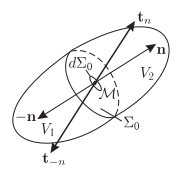
\includegraphics[width=0.7\linewidth]{img/que16}
	\caption{Внутренние поверхностные силы на площадке $\Sigma_0$}
	\label{fig:que16}
\end{wrapfigure}


Произвольную область $V$ разделим на две части $V_1$ и $V_2$ поверхностью $\Sigma_0$. Вектор нормали в точке $\mathcal{M}$ обозначим как $\mathbf{n}$, если он направлен в сторону $V_1$. На области $V_1$ и $V_2$ жействуют суммарные векторы внешних сил $\mathcal{F}_1$ и $\mathcal{F}_2$. Если рассмотреть элементарную площадку $d\Sigma \in \Sigma_0$, которой принадлежит рассматриваемая точка, то на ней действует поверхностная сила $d\mathcal{F}_1$ для области $V_1$ и $d\mathcal{F}_2$ для $V_2$. Обозначим плотности этих сил следующим образом:
\begin{equation*}
	\mathbf{t}_{n} = d\mathcal{F}_1 / d\Sigma \quad \text{и} \quad t_{-n} = d\mathcal{F}_2 / d\Sigma.
\end{equation*} 

Векторы $\mathbf{t}_n$ и $\mathbf{t}_{-n}$ называют \textit{векторами напряжений}, они представляют собой плотности \textit{внутренних поверхностных сил} по отношению ко всей области $V$ сплошной среды (так как они определены для внутренних точек $\mathcal{M}$ этой области).

  \que{Вектор напряжений. Теоремы 1 и 2 Коши о свойствах вектора напряжений.}

\paragraph{Вектор напряжений.} Как уже было отмечено в ответе на предыдущий вопрос, для некоторого разбиение области $V$ на $V_1$ и $V_2$ поверхностью $\Sigma_0$ имеем, что на некоторой элементарной площадке $d\Sigma \in \Sigma_0$ действуют поверхностные силы $d \mathcal{F}_1$ и $d \mathcal{F}_2$ для соответствующих областей. Тогда плотности этих сил можно обозначить следующим образом: 
\begin{equation*}
	\mathbf{t}_{n} = d\mathcal{F}_1 / d\Sigma \quad \text{и} \quad t_{-n} = d\mathcal{F}_2 / d\Sigma.
\end{equation*} 

Векторы $\mathbf{t}_n$ и $\mathbf{t}_{-n}$ называют \textit{векторами напряжений}, они представляют собой плотности \textit{внутренних поверхностных сил} по отношению ко всей области $V$ сплошной среды (так как они определены для внутренних точек $\mathcal{M}$ этой области). 

\paragraph{Теорема Коши о свойствах вектора напряжений.} Очевидна относительность разбиения сил на внешние и внутренние: одни и те же силы могут быть внутренними или внешними по отношению к различным объемам сплошной среды. 

Запишем уравнения изменения количества движения для всей области $V$ и для отдельных его частей $V_1$ и $V_2$:
\begin{align*}
	\int\limits_{V_1} \rho \left(\mathbf{f}_1 - \frac{d \mathbf{v}}{\mathbf{t}}\right) \, dV + \int\limits_{\Sigma_1} \mathbf{s}_1 \, d\Sigma + \int\limits_{\Sigma_0} \mathbf{t}_n \, d\Sigma &= 0, \\
	\int\limits_{V_2} \rho \left(\mathbf{f}_2 - \frac{d\mathbf{v}}{dt}\right) \, dV + \int\limits_{\Sigma_2} \mathbf{s}_2 \, d\Sigma + \int\limits_{\Sigma_0} \mathbf{t}_{-n} \, d\Sigma &= 0,
\end{align*}
где $\mathbf{f}_i$ и $\mathbf{s}_i$ --- силы, действующие в областях $V_i$ и на поверхностях $\Sigma_i$, т.е. $\mathbf{f} = \mathbf{f}_i$ в $V_i$ и $\mathbf{s} = \mathbf{s}_i$ на $\Sigma_i$. В силу непрерывности всех функций $\mathbf{s}_i$ и $\mathbf{f}_i$, вычитая их уравнения изменения количества движения уравнения для отдельных его частей получаем, что
\begin{equation*}
	\int\limits_{\Sigma_0} \left(\mathbf{t}_n + \mathbf{t}_{-n}\right) \, d\Sigma = 0.
\end{equation*}

В силу произвольности поверхности $\Sigma_0$, заключаем, что $\mathbf{t}_n + \mathbf{t}_{-n} = 0$. Таким образом, мы доказали следующую теорему. 

\begin{theorem*}[первая теорема Коши --- о непрерывности вектора напряжений]
	Для одной и той же точки $\mathcal{M}$, являющейся внутренней точкой области $V$, вектор напряжений, определенный по отношению к площадкам $\mathbf{n} \, d\Sigma_0$ и $-(\mathbf{n} \, d\Sigma_0)$, различается только знаком:
	\begin{equation*}
		\mathbf{t}_{n} = - \mathbf{t}_{-n},
	\end{equation*}
	т.е. поле $\mathbf{t}_n(x)$ --- непрерывно в области $V$.
\end{theorem*}

\begin{theorem*}[вторая теорема Коши]
	Вектор напряжений $\mathbf{t}_n$ на произвольной площадке с нормалью $\mathbf{n}$ выражается через векторы напряжений $\mathbf{t}_{\alpha}$ на трех координатных площадках следующим образом:
	\begin{equation*}
		\mathbf{t}_{n} = \sum\limits_{\alpha = 1}^{3} \mathbf{n} \cdot \mathbf{r}_{\alpha} \abs{\mathbf{r}^{\alpha}} \mathbf{t}_{\alpha}.
	\end{equation*}
	
	Т.к. 
	\begin{equation*}
		\abs{\mathbf{r}^{\alpha}} = \left(\mathbf{r}^{\alpha} \cdot \mathbf{r}^{\alpha}\right)^{1/2} = \sqrt{g^{\alpha\alpha}},
	\end{equation*}
	то соотношение из формулировки теоремы можно переписать в виде:
	\begin{equation*}
		\mathbf{t}_{n} = \mathbf{n} \cdot \mathbf{T},
	\end{equation*}
	где $\mathbf{T}$ --- тензор второго ранга, называемый \textit{тензором истинных напряжений Коши}:
	\begin{gather*}
		\mathbf{T} = \sum\limits_{\alpha = 1}^{3} \mathbf{r}_{\alpha} \otimes \mathbf{t}^{\alpha} = \mathbf{r}_{i} \otimes \mathbf{t}^i, \\
		\mathbf{t}^{\alpha} \equiv \mathbf{t}_{\alpha} \sqrt{g^{\alpha\alpha}}. 
	\end{gather*}
	
	Можно переформулировать теорему следующим образом: <<Для непрерывного в $V \cup \Sigma$ поля вектора напряжений $\mathbf{s}(x) = \mathbf{t}_n(x)$, удовлетворяющих уравнению закона изменения количества движения в интегральной форме, всегда существует поле тензора $\mathbf{T}(\mathbf{x})$, удовлетворяющее соотношению $\mathbf{t}_n = \mathbf{n} \cdot \mathbf{T}$ в $V \cup \Sigma$>>. 
\end{theorem*}
  \que{Тензор напряжений Коши, физический  смысл компонент тензора  напряжений Коши. Тензор напряжений Пиолы-Кирхгофа, физический  смысл компонент тензора  напряжений Пиолы-Кирхгофа.}

\paragraph{Тензор напряжений Коши и Пиолы-Кирхгофа.}

Тензор истинных напряжений Коши $\mathbf{T}$ определяется формулами:
\begin{gather*}
	\mathbf{T} = \sum\limits_{\alpha = 1}^{3} \mathbf{r}_{\alpha} \otimes \mathbf{t}^{\alpha} = \mathbf{r}_{i} \otimes \mathbf{t}^i, \\
	\mathbf{t}^{\alpha} \equiv \mathbf{t}_{\alpha} \sqrt{g^{\alpha\alpha}}, \\
	\mathbf{t}_{n} = \mathbf{n} \cdot \mathbf{T}.
\end{gather*}

Как и всякий тензор второго ранга его можно разложить по любому тензорному базису, например:
\begin{equation*}
	\mathbf{T} = T^{ij} \mathbf{r}_i \otimes \mathbf{r}_j = T_{ij} \mathbf{r}^{i} \otimes \mathbf{r}^{j}.
\end{equation*}

\begin{figure}[H]
	\centering
	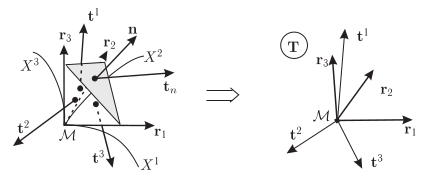
\includegraphics[width=0.6\linewidth]{img/que18}
	\caption{Геометрическое изображение тензора напряжений Коши}
	\label{fig:que18}
\end{figure}

Действительно, если выбрать векторы $\mathbf{r}_i$ в качестве левых векторов, а $\mathbf{t}^i$ рассматривать как правые векторы, то можно перейти к представлению тензора $\mathbf{T}$ в виде классов эквивалентности 
\begin{equation*}
	\mathbf{T} = \mathbf{r}_i \otimes \mathbf{t}^i = \left[\mathbf{r}_1 \mathbf{t}^1 \mathbf{r}_2 \mathbf{t}^2 \mathbf{r}_3 \mathbf{t}^3\right].
\end{equation*}

Тензор напряжений Коши $\mathbf{T}$ определен на площадке $d\Sigma$ в актуальной конфигурации (деформируемой площадке). Можно определить тензор напряжений и на соответствующей $d\mathring{\Sigma}$ в отсчетной конфигурации (недеформированной площадке). Для этого используем соотношение, связывающее $\mathcal{K}$ и $\mathring{\mathcal{K}}$:
\begin{equation*}
	\mathbf{n} d\Sigma = \sqrt{g / \mathring{g}} \, \mathring{\mathbf{n}} \cdot \mathbf{F}^{-1} \, d\mathring{\Sigma}_0,
\end{equation*} 
и рассмотрим вектор напряжений $\mathbf{t}_n$ на площадке $d\Sigma$:
\begin{equation*}
	\mathbf{t}_n \, d\Sigma = \mathbf{n} \cdot \mathbf{T} \, d\Sigma = \sqrt{g / \mathring{g}} \mathring{\mathbf{n}} \cdot \mathbf{F}^{-1} \cdot \mathbf{T} \, d\mathring{\Sigma} = \mathring{\mathbf{n}} \cdot \mathbf{P} \, d\mathring{\Sigma} = \mathring{\mathbf{t}}_n \, d\mathring{\Sigma}.
\end{equation*}

\begin{wrapfigure}[13]{l}{0.5\textwidth}
	\centering
	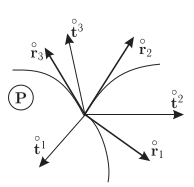
\includegraphics[width=0.45\linewidth]{img/que18_4}
	\caption{Геометрическое изображение тензора напряжений Пиолы-Кирхгофа $\mathbf{P}$}
	\label{fig:que18_4}
\end{wrapfigure}


Здесь введен тензор 
\begin{equation*}
	\mathbf{P} = \sqrt{g / \mathring{g}} \, \mathbf{F}^{-1} \cdot \mathbf{T},
\end{equation*}
называемый \textit{первым тензором напряжений Пиолы-Кирхгофа}, который очевидно определен на недеформированной площадке $d\mathring{\Sigma}$. 

Вектор $\mathring{\mathbf{t}}_n$ называют \textit{вектором напряжений Пиолы-Кирхгофа}, он связан с тензором $\mathbf{P}$ формулой Коши:
\begin{equation*}
	\mathring{\mathbf{t}}_n = \mathring{\mathbf{n}} \cdot \mathbf{P}.
\end{equation*}

Выражение можно представить в виде классов эквивалентности:
\begin{equation*}
	\mathbf{P} = \mathring{\mathbf{r}}_i \otimes \mathring{\mathbf{t}}^i = \left[\mathring{\mathbf{r}}_1 \mathring{\mathbf{t}}^1 \mathring{\mathbf{r}}_2 \mathring{\mathbf{t}}^2 \mathring{\mathbf{r}}_3 \mathring{\mathbf{t}}^3\right], 
\end{equation*}
где обозначены векторы
\begin{equation*}
	\mathring{\mathbf{t}}^{\alpha} = \mathbf{t}_{\alpha} \sqrt{g^{\alpha \alpha} g / \mathring{g}}.
\end{equation*}

С помощью этого представления можно также дать геометрическое изображение тензора Пиолы-Кирхгофа в базисе $\mathring{\mathbf{r}}_i$ отсчетной конфигурации.

\paragraph{Физический смысл компонент тензора Коши.}


\begin{wrapfigure}[19]{l}{0.5\textwidth}
	\centering
	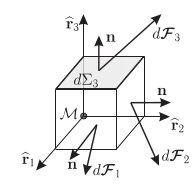
\includegraphics[width=0.7\linewidth]{img/que18_2}
	\caption{К вопросу о физическом смысле компонент тензора напряжений Коши}
	\label{fig:que18_2}
\end{wrapfigure}

Пусть в $\mathcal{K}$ имеется локальный базис $\mathbf{r}_i$, мы всегда можем построить ортогональный базис $\widetilde{\mathbf{r}}_i$, а затем, нормируя, ортонормированный $\widehat{\mathbf{r}}_i$, который мы называем \textit{физическим базисом}. В этом базисе тензор напряжений Коши имеет компоненты $\widehat{T}^{ij}$, совпадающие с $\widehat{T}_{ij}$: 
\begin{equation*}
	\mathbf{T} = \widehat{T}^{i j} \widehat{\mathbf{r}}_i \otimes \widehat{\mathbf{r}}_j.
\end{equation*}
Выберем теперь произвольную материальную точку $\mathcal{M} \in V$ и рассмотрим элементарный объем $dV \in V$, содержащий эту точку и имеющий форму куба, грани которого ортогональны векторам $\widehat{\mathbf{r}}_{\alpha}, \, \alpha 1, 2, 3$. Поскольку мы рассматриваем элементарный объем $dV$, то тензор напряжений $\mathbf{T}(x)$ одинаков в каждой точке $\mathbf{x} \in dV$ и $d\Sigma_{\alpha}$, $\alpha = 1, 2, 3$. 

На каждой грани $d\Sigma_{\alpha}$ действует поверхностная сила $d\mathcal{F}_{\alpha}$, связанная с вектором напряжений $\mathbf{t}_{n}$ на этой грани соотношениями плотности внутренних поверхностных сил:
\begin{equation*}
	\text{на } d\Sigma_{\alpha}: \quad \frac{d \mathcal{F}_{\alpha}}{d \Sigma_{\alpha}} = \mathbf{t}_n = \mathbf{n} \cdot \mathbf{T}.
\end{equation*}

Представляя векторы $d\mathcal{F}_{\alpha}$ и $\mathbf{n}$ в базисе $\widehat{\mathbf{r}}_i$:
\begin{equation*}
	d\mathcal{F}_{\alpha} = d\tensor{\mathcal{F}}{^i_{\alpha}} \widehat{\mathbf{r}}_i, \quad \mathbf{n} = \widehat{n}^i \widehat{\mathbf{r}}_i,
\end{equation*}
получаем: 
\begin{equation*}
	\text{на } d\Sigma_{\alpha}: \quad \frac{d\tensor{\mathcal{F}}{^i_{\alpha}}}{d\Sigma_{\alpha}} = \widehat{n}_j \widehat{T}^{ji} = \widehat{T}^{\alpha i}, \quad \alpha = 1, 2, 3,
\end{equation*}
так как на $d\Sigma_{\alpha}: \widehat{n}_{\beta} = \widehat{n}_{\gamma} = 0, \, \alpha \not = \beta \not = \gamma \not = \alpha$. 

Это позволяет прояснить физический смысл компонент $\widehat{T}^{ij}$ тензора напряжений Коши:
\begin{equation*}
	\text{на } d\Sigma_{\alpha}: \quad \widehat{T}^{\alpha\alpha} = \frac{d \mathcal{F}^{\alpha}_{\alpha}}{d\Sigma_{\alpha}}, \, \widehat{T}^{\alpha\beta} = \frac{d\mathcal{F}^{\beta}_{\alpha}}{d\Sigma_{\alpha}}, \, \widehat{T}^{\alpha \gamma} = \frac{d \mathcal{F}^{\gamma}_{\alpha}}{d\Sigma_{\alpha}}, \, \alpha \not = \beta \not = \gamma \not = \alpha.
\end{equation*}

\textit{Нормальные напряжения} $\widehat{T}^{\alpha \alpha}$ --- это отношение соответствующей нормальной компоненты $d\mathcal{F}^{\alpha}_{\alpha}$
 поверхностной силы $d\mathcal{F}_{\alpha}$, действующей на площадке $d\Sigma_{\alpha}$, к величине этой площадки, а \textit{касательные напряжения} $\widehat{T}^{\alpha \beta}, \widehat{T}^{\alpha \gamma}$ --- это отношения касательных компонент $d\mathcal{F}^{\beta}_{\alpha}, d\mathcal{F}^{\gamma}_{\alpha}$ той же силы $d\mathcal{F}_{\alpha}$, действующей на площадке $d\Sigma_{\alpha}$, к величине этой же площадки.

\begin{remark*}
	Поскольку $\mathbf{T}$ одинаков во всем кубе $dV$, то, вследствии первой теоремы Коши, силы $d\mathcal{F}_{\alpha}$ на противоположных гранях куба отличаются только знаком, поэтому соотношения для нормальных и касательных напряжений одни и те же. 
\end{remark*}

\begin{remark*}
	В силу сказанного, различных соотношений --- по три на каждой из трех граней $d\Sigma_{\alpha}$, т.е. всего девять соотношений: для трех нормальных напряжений $\widehat{T}^{\alpha \alpha}$ и шести касательных напряжений $\widehat{T}^{\alpha \beta}, \, \alpha \not = \beta$. 
\end{remark*}

\paragraph{Физический смысл компонент тензора Пиола-Кирхгофа.}

В ортонормированном базисе $\widehat{\mathring{\mathbf{r}}}_i$ отсчетной конфигурации:
\begin{equation*}
	\mathbf{P} = \widehat{P}^{ij} \widehat{\mathring{\mathbf{r}}}_i \otimes \widehat{\mathring{\mathbf{r}}}_j.
\end{equation*}

Выберем в $\mathring{\mathcal{K}}$ материальную точку $\mathcal{M}$ и рассмотрим элементарный объем $d\mathring{V}$ в форме куба, содержащий эту точку. Грани куба $d\mathring{\Sigma}_{\alpha}$, как и ранее, выберем ортогональными векторам $\widehat{\mathring{\mathbf{r}}}_{\alpha}$.

Этому кубу $d\mathring{V}$ в конфигурации $\mathcal{K}$ соответствует искаженный объем $dV$. В силу геометрической картины преобразования материальной точки сплошной среды, объем $dV$ будет иметь форму параллелепипеда, вообще говоря, с наклонными гранями $d\Sigma_{\alpha}$, но остающимися плоскими.

\begin{figure}[H]
	\centering
	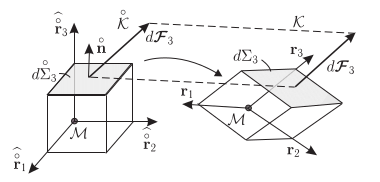
\includegraphics[width=0.6\linewidth]{img/que18_3}
	\caption{К вопросу о физическом смысле компонент тензора напряжений Пиолы-Кирхгофа}
	\label{fig:que18_3}
\end{figure}

 Для элементарных объемов $d\mathring{V}$ и $dV$ тензоры напряжений $\mathbf{T}(\mathbf{x})$ и $\mathbf{P}(\mathring{\mathbf{x}})$ одинаковы в каждой точке $\mathbf{x} \in \overline{dV}$ и $\mathring{\mathbf{x}} \in \mathring{\overline{dV}}$. 
 
 На деформированной (но плоской) грани $d\Sigma_{\alpha}$ действует поверхностная сила $d\mathcal{F}_{\alpha}$. Перенесем ее параллельным переносом в $\mathring{\mathcal{K}}$ на соответствующую грань $d\mathring{\Sigma}_{\alpha}$, тогда на грани $d\mathring{\Sigma}_{\alpha}$ можно записать следующие соотношения:
 \begin{equation*}
 	\text{на } d\mathring{\Sigma}_{\alpha} : \quad \frac{d\mathcal{F}_{\alpha}}{d\Sigma_{\alpha}} \left(\frac{d\Sigma_{\alpha}}{d\mathring{\Sigma}_{\alpha}}\right) = \mathbf{t}_n \left(\frac{d\Sigma_{\alpha}}{d\mathring{\Sigma}_{\alpha}}\right) = \mathring{\mathbf{n}} \cdot \mathbf{P}.
 \end{equation*}
 
 Представляя векторы $d\mathcal{F}_{\alpha}$ и $\mathring{\mathbf{n}}$ в базисе $\widehat{\mathring{\mathbf{r}}}_i$: 
 \begin{equation*}
 	d\mathcal{F}_{\alpha} = d\tensor{\mathring{\mathcal{F}}}{^i_{\alpha}} \widehat{\mathring{\mathbf{r}}}_i, \quad \mathring{\mathbf{n}} = \widehat{\mathring{n}}^i \widehat{\mathring{\mathbf{r}}}_i,
 \end{equation*}
 и из соотношений на $d\mathring{\Sigma}_{\alpha}$ получаем:
 \begin{equation*}
 	\text{на } d\mathring{\Sigma}_{\alpha} : \quad \frac{d\tensor{\mathring{\mathcal{F}}}{^i_{\alpha}}}{d\Sigma_{\alpha}} = \widehat{\mathring{n}} \widehat{P}^{ij} = \widehat{P}^{\alpha i}, \quad \alpha = 1, 2, 3, 
 \end{equation*}
 т.к. на $\mathring{\Sigma}_{\alpha} : \widehat{\mathring{n}}_\alpha = 1$, а $\widehat{\mathring{n}}_{\beta} = \widehat{\mathring{n}}_{\gamma} = 0$. 

Итого, получаем:
\begin{equation*}
	\text{на } d\mathring{\Sigma}_{\alpha} : \quad \widehat{P}^{\alpha\alpha} = \frac{d\mathring{\mathcal{F}}^{alpha}_{\alpha}}{d\mathring{\Sigma}_{\alpha}}, \quad \widehat{P}^{\alpha \beta} = \frac{d \mathring{\mathcal{F}}^{\beta}_{\alpha}}{d\mathring{\Sigma}_{\alpha}}, \quad \widehat{P}^{\alpha \gamma} = \frac{d \mathring{\mathcal{F}}^{\gamma}_{\alpha}}{d\mathring{\Sigma}_{\alpha}}, \quad \alpha \not = \beta \not = \gamma \not = \alpha.
\end{equation*}

Таким образом, \textit{нормальное напряжение} $\widehat{P}^{\alpha \alpha}$ --- это отношение нормальной компоненты $d\mathring{\mathcal{F}}^{\alpha}_{\alpha}$ поверхностной силы $d\mathcal{F}_{\alpha}$, действующей на деформированной площадке $d\Sigma_{\alpha}$, к величине соответствующей недеформированной площадке $d\mathring{\Sigma}_{\alpha}$. \textit{Касательные напряжения} $\widehat{P}^{\alpha\beta}, \widehat{P}^{\alpha\gamma}$ --- это отношения касательных компонент $d\mathring{\mathcal{F}}^{\beta}_{\alpha}, d\mathring{\mathcal{F}}^{\gamma}_{\alpha}$ той же поверхностной силы $d\mathcal{F}_{\alpha}$, действубщей на деформированной площадке $d\Sigma_{\alpha}$, к величине недеформированной площадки $d\mathring{\Sigma}_{\alpha}$.

Замечания для $\mathbf{T}$ остаются справедливыми и для $\mathbf{P}$. За исключением того, что тензор $\mathbf{P}$ остается несимметричным, даже если $\mathbf{T}$ --- симметричен. 
  \que{Уравнение  движения  в  пространственном и материальном описании.}

Подставляя 
\begin{equation*}
	\mathbf{t}_{n} = d\mathcal{F}_1 / d\Sigma \quad \text{и} \quad t_{-n} = d\mathcal{F}_2 / d\Sigma.
\end{equation*}

в
\begin{equation*}
	\mathbf{t}_n = \mathbf{n} \cdot \mathbf{T},
\end{equation*}

получим:
\begin{equation*}
	\frac{d}{dt} \int\limits_{V} \rho \mathbf{v} \, dV = \int\limits_{\Sigma} \mathbf{n} \cdot \mathbf{T} \, d\Sigma + \int\limits_{V} \rho \mathbf{f} \, dV.
\end{equation*}

Теперь подставим все то же в \eqref{omega} (вопрос №16):
\begin{equation*}
	\int\limits_{V} \left(\rho \frac{d\mathbf{v}}{dt} - \rho \mathbf{f}\right) = \int\limits_{\Sigma} \mathbf{n} \cdot \mathbf{T} \, d\Sigma,
\end{equation*}
и преобразуя поверхностный интеграл к объемному по формуле Гаусса-Остроградского, придем к следующему соотношению:
\begin{equation*}
	\int\limits_{V} \left(\rho \frac{d \mathbf{v}}{dt} - \rho \mathbf{f} - \nabla \cdot \mathbf{T}\right) \, dV = 0.
\end{equation*}

Отсюда, в силу произвольности объема $V$, заключаем, что подынтегральное выражение должно всегда обращаться в ноль. Итак мы доказали следующую теорему.

\begin{theorem*}
	Если функции $\mathbf{F}$, $\mathbf{v}$, $\mathbf{T}$ и $\mathbf{f}$, удовлетворяющие закону изменения количества движения и зависящие от $x^i$, $t$ являются непрерывно-дифференцируемыми в $V(t)$ для всех рассматриваемых $t \geqslant 0$, то в каждой точке $\mathcal{M} \in V(t)$ имеет место \textbf{уравнение движения в эйлеровом описании} (т.е. в $\mathcal{K}$):
	\begin{equation*}
		\rho \frac{d\mathbf{v}}{dt} = \nabla \cdot \mathbf{T} + \rho \mathbf{f}.
	\end{equation*}
\end{theorem*}


Используя свойство полной производной, уравнение движения можно записать в \textit{дивергентной форме}:
\begin{equation*}
	\frac{\partial \rho \mathbf{v}}{\partial t} + \nabla \cdot \rho \mathbf{v} \otimes \mathbf{v} = \nabla \cdot \mathbf{T} + \rho \mathbf{f}.
\end{equation*}

Преобразуем теперь уравнение движения:
\begin{equation*}
	\int\limits_{\mathring{V}} \mathring{\rho} \left(\frac{d\mathbf{v}}{dt} - \mathbf{f}\right) \, d\mathring{V} - \int\limits_{\mathring{\Sigma}} \mathring{\mathbf{n}} \cdot \mathbf{P} \, d\mathring{\Sigma} = 0. 
\end{equation*}

С помощью теоремы Гаусса-Остроградского преобразуем это уравнение к виду:
\begin{equation*}
	\int\limits_{\mathring{V}} \left(\mathring{\rho} \left(\frac{d\mathbf{v}}{dt} - \mathbf{f}\right) - \mathring{\nabla} \cdot \mathbf{P}\right) \, d\mathring{V} = 0.
\end{equation*}

Откуда в силу произвольности объема $\mathring{V}$, получаем еще одну теорему. 

\begin{theorem*}
	Если выполнены условия предыдущей теоремы, то в каждой точке $\mathcal{M} \in \mathring{V}$ для всех рассматриваемых $t \geqslant 0$ имеет место \textbf{уравнение движения в лагранжевом (материальном) описании} (т.е в $\mathring{\mathcal{K}}$):
	\begin{equation*}
		\mathring{\rho} \frac{d\mathbf{v}}{dt} = \mathring{\rho} \mathbf{f} + \mathring{\nabla} \cdot \mathbf{P}.
	\end{equation*}
	
	Так как в лагранжевом описании полная производная по времени совпадает с частной, то дивергентная форма уравнения движения в $\mathring{\mathcal{K}}$ совпадает с приведенной выше формулой:
	\begin{equation*}
		\mathring{\rho} \frac{\partial\mathbf{v}}{\partial t} = \mathring{\rho} \mathbf{f} + \mathring{\nabla} \cdot \mathbf{P}.
	\end{equation*}
\end{theorem*}

  \que{Закон сохранения моментов количества движения. Обобщенная теорема Коши. Дифференциальная форма закона сохранения моментов количества движения. Полярные и неполярные среды. Симметрия тензора напряжений Коши.}

  \que{Первый закон термодинамики в пространственном и материальном описании. Интегральная и дифференциальная формулировки. Вектор потока тепла. }

  \que{Второй закон термодинамики в пространственном и материальном описании. Интегральная и дифференциальная формулировки. }

  \que{Понятие о коэффициенте полезного действия.}

  \que{Статические уравнения совместности деформаций. Четыре различные формулировки.}

  \que{Динамические уравнения совместности деформаций в материальном и пространственном описании.}

  \que{Полные системы законов сохранения в пространственном и материальном описании.}


  % Теория определяющих соотношений
  \que{Незамкнутость системы законов сохранений МСС. Понятие об определяющих соотношениях. Принципы построения определяющих соотношений. Основное термодинамическое тождество.}
\footnote{Димитриенко Ю.И. -- Нелинейная механика сплошных сред, стр. 149}

\paragraph{Незамкнутость системы законов сохранений МСС.}
Полная система законов сохранения в полных дифференциалах:
\begin{equation*}
  \begin{cases}
    \rho \dfrac{d \bar{A}_\alpha}{dt} = \nabla \cdot \bar{B}_\alpha + \rho C_\alpha, 
    \alpha = 1..6 \\

    \bar{A}_\alpha = \begin{pmatrix}
      1/\rho \\ \mathbf{v} \\ e + |v|^2 / 2 \\ \eta \\ \mathbf{u} \\ \mathbf{F}^T
    \end{pmatrix}, \quad

    \bar{B}_\alpha = \begin{pmatrix}
      \mathbf{v} \\ \mathbf{T} \\ \mathbf{T} \cdot \mathbf{v} - \mathbf{q} \\ -\mathbf{q} / \theta \\
      \mathbf{0} \\ \rho \mathbf{F} \otimes \mathbf{v}
    \end{pmatrix}, \quad

    C_\alpha = \begin{pmatrix}
      0 \\ \mathbf{f} \\ \mathbf{f} \cdot \mathbf{v} + q_m \\ 
      (q_m + q^*) / \theta \\ 
      \mathbf{v} \\ \mathbf{0}
    \end{pmatrix} 
  \end{cases}
\end{equation*}
данная система содержит 18 скалярных уравнений и 29 скалярных неизвестных
$\rho, \mathbf{v}, \mathbf{u}, \mathbf{T}, e, \eta, \theta, \mathbf{q}, \mathbf{F}, q^*$.
Эта система одинакова для любой сплошной среды.

\paragraph{Определяющие соотношения.}
Для замыкания системы уравнений необходимы дополнительные соотношения. Эти дополнительные
соотношения называют \emph{определяющими соотношениями}, поскольку именно они определяют, чем одна
сплошная среда отличается от другой (универсальные законы сохранения «не различают» типы
сплошных сред — они одинаковы для всех тел). Если заданы каким-либо образом определяющие
соотношения, то говорят, что задана \emph{модель сплошной среды}.

\paragraph{Принципы построения ОС.}
Вывод определяющих соотношений основан на привлечении некоторых дополнительных принципов,
т.е. физических допущений общего характера, которые, вообще говоря, не формулируются в виде
дифференциальных уравнений в частных производных. Основными такими принципами являются:
\begin{itemize}
  \item принцип термодинамически согласованного детерминизма,
  \item принцип локальности,
  \item принцип равноприсутствия,
  \item принцип материальной индифферентности (объективности),
  \item принцип материальной симметрии,
  \item принцип Онзагера.
\end{itemize}
Кроме того, для частных моделей сред формулируют дополнительные принципы.

\paragraph{Основное термодинамическое тождество.}
% TODO Нелинейный Димитриенко, стр 177.
Выпишем законы изменения энергии и закон притока тепла в полных дифференциалах:
\[
  \begin{cases}
    \rho \dfrac{de}{dt} =
    \mathbf{T} \cdot\cdot(\nabla \otimes \mathbf{v})^T +
    \rho q_m - \nabla\cdot\mathbf{q}, \\
    \rho\theta \dfrac{d\eta}{dt} =
    \rho q_m - \nabla \cdot \mathbf{q} + w^*,
  \end{cases}
\]
исключая $\nabla \cdot \mathbf{q}$ из этих уравнений, и вспоминая обозначение $w_{(i)} = \mathbf{T} \cdot\cdot (\nabla \otimes \mathbf{v})^T$, получим:
\[
  \rho \left( \dfrac{de}{dt} - \theta \dfrac{d\eta}{dt} \right) - w_{(i)} + w^* = 0.
\]

Сюда вместо $w_{(i)}$ можно подставить выражение через энергетические пары тензоров
(см. следующий вопрос), и тогда
это соотношение можно мыслить себе как некоторое соотношение, связывающее изменение трёх
основных величин: $e, \theta$ и $\stackrel{(n)}{\mathbf{C}}$
(или $e, \theta$ и $\stackrel{(n)}{\mathbf{G}}$,
или $e, \theta, \stackrel{(n)}{\mathbf{A}}$ и $\mathbf{O}^T$, 
или $e, \theta, \stackrel{(n)}{\mathbf{g}}$ и $\mathbf{O}^T$)
в локальной точке сплошной среды.

Различают также $e$- и $\psi$-формы ОТТ, то выражение, которое написано выше, называют $e$-формой,
потому что оно содержит энергию $e$. Если ввести т.н. \emph{свободную энергию Гельмгольца} 
$\psi = e - \theta \eta$, то получим выражение в $\psi-$ форме:
\[
  \rho \dfrac{d\psi}{dt} + \rho\eta \dfrac{d\theta}{dt} - w_{(i)} + w^* = 0.
\]

Вообще говоря, ОТТ можно записать ещё в 100 других видах, вводя всё новые и новые (и никому не
нужные) замены, но важно, что в ОТТ некоторые переменные входят через производные -- такие
будет называть \emph{реактивными} $\mathcal{R}$, а другие назовём \emph{активными} $\Lambda$.

  \que{Энергетические пары тензоров напряжений и деформаций. }
В законе изменения кинетической энергии использовалась величина $W_{(i)}$ -- мощность внутренних
поверхностных сил, которую мы определяли как
$W_{(i)} = - \int_V \mathbf{T} \cdot\cdot (\nabla \otimes \mathbf{v})^T \, dV$.
Обозначим $w_{(i)} = \mathbf{T} \cdot\cdot (\nabla \otimes \mathbf{v})^T$ --
\emph{мощность напряжений}, тогда $W_{(i)} = - \int_V w_{(i)} \, dV$.

\begin{definition}[\footnote{Димитриенко -- Нелинейная МСС, стр 150}]
  \emph{Энергетическими тензорами напряжений} $\stackrel{(n)}{\mathbf{T}}$,
  и \emph{энергетическими тензорами деформаций} $\stackrel{(n)}{\mathbf{C}}$
  называются такие пары тензоров, которыми наиболее удачно можно представить мощность напряжений
  в виде:
  \[
    w_{(i)} = \stackrel{(n)}{\mathbf{T}} \cdot\cdot \dfrac{d}{dt} \stackrel{(n)}{\mathbf{C}} + \mathbf{T}^K \cdot\cdot \mathbf{W},
  \]
  где $T^K = \dfrac{1}{2} (T - T^T)$ -- кососиметричная часть тензора напряжений Коши $T$, а 
  $\mathbf{W}$ -- тензор вихря.

  В случаях, когда $T = T^T$, второе слагаемое отсутствует.
\end{definition}

Выделяют 5 пар таких тензоров.

\begin{center}
  \begin{tabular}{|c|c|c|}
    \hline
    $n$ & $\stackrel{(n)}{\mathbf{T}}$ & $\stackrel{(n)}{\mathbf{C}}$ \\
    \hline
    I & $\mathbf{F}^T \cdot \mathbf{T}^S \cdot \mathbf{F}$ & $\boldsymbol{\Lambda} = \dfrac{1}{2} (\mathbf{E} - \mathbf{U}^{-2})$ \\
    II & $1/2 (\mathbf{F}^T \cdot \mathbf{T}^S \cdot \mathbf{O} + \mathbf{O}^T \cdot \mathbf{T}^S \cdot \mathbf{F})$ & $\mathbf{E} - \mathbf{U}^{-1}$ \\
    III & $\mathbf{O}^T \cdot \mathbf{T}^s \cdot \mathbf{O}$ & $\mathbf{B}$ \\
    IV & $1/2 (\mathbf{F}^{-1} \cdot \mathbf{T}^s \cdot \mathbf{O} + \mathbf{O}^T \cdot \mathbf{T}^S \cdot \mathbf{F}^{-1T})$ & $\mathbf{U} - \mathbf{E}$ \\
    V & $\mathbf{F}^{-1} \cdot \mathbf{T}^S \cdot \mathbf{F}^{-1T}$ & $\mathbf{C} = \dfrac{1}{2}(\mathbf{U}^2 - \mathbf{E})$ \\
    \hline
  \end{tabular}
\end{center}
где $T^S = \dfrac{1}{2} (T + T^T)$ - симметрическая часть тензора напряжений Коши;
$\mathbf{F}$ -- тензор градиента деформаций;
$\mathbf{O}, \mathbf{U}$ -- полярное разложение тензора градиента деформаций $\mathbf{F} = \mathbf{O} \cdot \mathbf{U}$.

% В случае третьей пары, энергетический тензор деформаций $\stackrel{(III)}{\mathbf{C}} = \mathbf{B}$
% неизвестен, но является решением следующего ДУ

% TODO проверить, что ещё можно написать.


  \que{Принцип термодинамически согласованного детерминизма, принцип локальности.}

\paragraph{Аксиома принцип термодинамически согласованного детерминизма.}
Для любой сплошной среды активные переменные $\Lambda$ полностью определяются реактивными
переменными $\mathcal{R}$, иначе говоря, существует отображение обобщенного пространства
реактивных переменных $\chi_{\mathcal{R}}$ в пространсвто активных переменных $\chi_\Lambda$:
\begin{equation}
  \breve{f} : \chi_{\mathcal{R}} \to \chi_\Lambda,
\end{equation}
которое называют \emph{операторным соотношением (оператором)} и записывают в виде
\begin{equation}\label{thermodinamic-determinizm-principle}
  \Lambda = \breve{f} (\mathcal{R})
\end{equation}
, причём это соотношение <<согласовано с термодинамикой>>,
т.е. тождественно удовлетворяет ОТТ.

\begin{remark}
  Соотношение \eqref{thermodinamic-determinizm-principle} вообще говоря, просто
  устанавливает существование некоторой зависимости между этими наборами переменных, однако, это
  совсем не означает, что $\Lambda(t)$ зависит только от $\mathcal{R}(t)$.
\end{remark}

\paragraph{Принцип локальности.} Для всякой сплошной среды операторы
определяющих соотношений в любой из форм \eqref{thermodinamic-determinizm-principle} таковы, что
активные переменные в любой материальной точке зависят только от реактивных переменных в этой же
точке.


  \que{Общий вид определяющих соотношений сплошных сред  (модели  An ).  Определение идеальных сред. Общий вид определяющих соотношений для идеальных сплошных сред.}

  \que{Н-преобразования отсчетной конфигурации. Понятие об H-индифферентных и Н-инвариантных тензорах, примеры.}

  \que{Группы симметрии сплошной среды. Принцип материальной симметрии. Определение жидких и твердых сред.}

  \que{Основные группы симметрии твердых сред: группы изотропии, трансверсальной изотропии и ортотропии. Н-индифферентные функции относительно групп симметрии.}

\begin{definition*}
	Твердое тело называют \textit{изотропным}, если его группа симметрии $\hat{G}_s$ в неискаженной конфигурации $\hat{\mathcal{K}}$ совпадает с $I$:
	\begin{equation*}
		\hat{G}_s = I.
	\end{equation*}
\end{definition*}

Четыре наиболее широко используемые в МСС подгруппы:
\begin{itemize}
	\item триклинная группа $\hat{G}_s = E$ (точечная, состоит из 2 элементов), 
	
	\item группа ортотропии $\hat{G}_s = O$ (точечная, состоит из 8 элементов), 
	
	\item группа трансверсальной изотропии $\hat{G}_s = T_3$ (непрерывная),
	
	\item группа изотропии (полная ортогональная) $\hat{G}_s = I$ (непрерывная). 
\end{itemize}

\begin{definition*}
	Тензор $\Omega$, заданный в конфигурации $\mathring{\mathcal{K}}$, называют $H$-индифферентным относительно группы $\mathring{G}_s \subset I$, если для любого ортогонального тензора преобразования $\overset{\ast}{\mathbf{Q}} : \mathring{\mathcal{K}} \to \overset{\ast}{\mathcal{K}}$ из этой группы, то он удовлетворяет условию:
	\begin{equation*}
		\overset{\ast}{\Omega} = \overset{\ast}{\mathbf{Q}}^{T} \cdot \Omega \cdot \overset{\ast}{\mathbf{Q}}, \quad \forall \overset{\ast}{\mathbf{Q}} \in \mathring{G}_s.
	\end{equation*}
	
	Иначе говоря, существуют тензоры, $H$-индефферентные относительно только определенных подгрупп ортогональной группы; тензоры же, которые $H$-индифферентны относительно любых $H$-преобразований будем называть \textit{абсолютно} $H$-\textit{индифферентными}.
\end{definition*}
  \que{Инварианты тензоров 2-го ранга относительно произвольной группы симметрии, функциональные базисы инвариантов. }

  \que{Инварианты тензоров 2-го ранга относительно  групп  изотропии, трансверсальной изотропии и ортотропии. Анизотропные среды, примеры. }

  \que{Представления определяющих соотношений для идеальных твердых сред c помощью инвариантов (случаи изотропии, трансверсальной изотропии, ортотропии).}


\end{document}
